\chapter{Testing for Verification}
\label{chap:verification}

\section{Verification strategy}
\label{sec:verification_strategy}

This chapter documents the test cases used to verify the correctness and consistency of the implemented Gray--Scott solver. The focus is on \emph{verification}, i.e.\ checking whether the numerical methods and their implementation solve the intended discrete problem correctly. In accordance with the PPP guideline, the chapter therefore emphasizes reproducible test cases with clearly defined aims, setups, execution procedures, expected results, and obtained results.

The verification strategy is organized in several layers. First, low-level operator tests are used to verify the correctness and convergence of the discrete diffusion operator. Second, time-integration tests check whether the explicit Euler method shows the expected temporal behavior. Third, boundary-condition tests confirm that Dirichlet and Neumann boundary conditions are imposed correctly in the implemented formulations. Fourth, equivalence tests compare different implementation variants, especially the matrix-based and stencil-based diffusion operators, in order to verify that they produce consistent results. Finally, interface-level consistency tests are used to check that the GUI execution path reproduces the same numerical results as the non-GUI reference workflow.

Besides these formal verification tests, the project also includes a validation-oriented pattern sanity check based on a Pearson-type Gray--Scott setup. This test is not a strict proof of numerical correctness in the sense of manufactured-solution verification, but it provides an additional qualitative sanity check that the implemented model reproduces physically plausible pattern-forming behavior. Since validation is not mandatory in the PPP guideline, such tests are treated here as supportive evidence rather than as the main verification basis.

Overall, the chapter is designed to move from rigorous numerical verification of core building blocks toward consistency checks of the full implementation. This layered structure is important because correctness of the final simulation results depends not only on the governing equations, but also on the correct interaction of operator assembly, time stepping, boundary treatment, solver implementation, and user interface execution.

\section{Detailed Verification Test Cases}
\label{sec:verification_detailed_cases}

\subsection{Test Case 1: MMS operator convergence of the discrete Laplacian}
\label{sec:verification_testcase_mms_operator}

\paragraph{Aim.}
This test case verifies the spatial accuracy of the discrete Laplacian operator implemented in the code. The purpose is to check that the matrix-based finite-difference Laplacian produced by \texttt{buildLaplacian2D} converges with the expected second-order accuracy on a sequence of refined grids when it is applied to a smooth exact solution. Since the Laplacian operator is one of the core building blocks of the Gray--Scott solver, this is a fundamental verification step.

\paragraph{Setup.}
The test uses the Method of Manufactured Solutions (MMS). A smooth periodic exact solution is prescribed on the square domain
\[
\Omega = [0,1)\times[0,1)
\]
with periodic boundary conditions in both spatial directions. The manufactured fields are
\[
u^\ast(x,y,t) = 1.0 + 0.1\cos\!\bigl(2\pi(2x+3y)+t\bigr),
\]
\[
v^\ast(x,y,t) = 0.5 + 0.1\cos\!\bigl(2\pi(2x+3y)+t\bigr).
\]
The corresponding exact Laplacians are known analytically:
\[
\nabla^2 u^\ast(x,y,t) = -0.1(2\pi)^2(2^2+3^2)\cos\!\bigl(2\pi(2x+3y)+t\bigr),
\]
\[
\nabla^2 v^\ast(x,y,t) = -0.1(2\pi)^2(2^2+3^2)\cos\!\bigl(2\pi(2x+3y)+t\bigr).
\]

The test evaluates the operator at the fixed time
\[
t_0 = 0.3.
\]
Uniform grids with
\[
N_x=N_y\in\{32,64,128,256\}
\]
are used. Since \(L_x=L_y=1\), the grid spacing is
\[
h = \frac{1}{N}.
\]

For each grid, the sparse discrete Laplacian matrix \(L\) is assembled and applied to the exact grid values of \(u^\ast\) and \(v^\ast\). The numerical result is compared against the analytic Laplacian, and the discrete \(L^2\) error is computed.

\paragraph{How to run the test case.}
From the project \texttt{tests} folder, run:
\begin{verbatim}
r = test_mms_operator_convergence();
\end{verbatim}

The test prints the error values in the MATLAB command window and saves the convergence plot in the local output folder of
\begin{verbatim}
tests/test_case_01_mms_operator/
\end{verbatim}

\paragraph{Expected result.}
For a smooth periodic solution on a uniform grid, the standard five-point finite-difference Laplacian is expected to be second-order accurate in space. Therefore, the discrete \(L^2\) error should satisfy
\[
\|L u^\ast - \nabla^2 u^\ast\|_{L^2} = \mathcal{O}(h^2),
\qquad
\|L v^\ast - \nabla^2 v^\ast\|_{L^2} = \mathcal{O}(h^2).
\]
As a consequence, halving the grid spacing should reduce the error by approximately a factor of four. On a log--log plot of error versus \(h\), the measured slope should be close to \(2\).

\paragraph{Obtained result.}
The test produced the error values listed in Table~\ref{tab:mms_operator_convergence_data}. The corresponding convergence plot is shown in Fig.~\ref{fig:mms_operator_convergence}.

\begin{table}[htbp]
\centering
\caption{Measured \(L^2\) errors for the discrete Laplacian MMS operator test.}
\label{tab:mms_operator_convergence_data}
\begin{tabular}{|c|c|c|c|}
\hline
\(N_x=N_y\) & \(h\) & \(\|L u^\ast - \nabla^2 u^\ast\|_{L^2}\) & \(\|L v^\ast - \nabla^2 v^\ast\|_{L^2}\) \\
\hline
32  & 0.03125   & \(8.609\times 10^{-1}\) & \(8.609\times 10^{-1}\) \\
64  & 0.015625  & \(2.169\times 10^{-1}\) & \(2.169\times 10^{-1}\) \\
128 & 0.0078125 & \(5.434\times 10^{-2}\) & \(5.434\times 10^{-2}\) \\
256 & 0.00390625 & \(1.359\times 10^{-2}\) & \(1.359\times 10^{-2}\) \\
\hline
\end{tabular}
\end{table}

The observed convergence orders reported by the code are
\[
p_u = 2.00, \qquad p_v = 2.00.
\]
This exactly matches the theoretical expectation for a second-order finite-difference Laplacian. In addition, the error decreases by approximately a factor of four whenever the grid is refined by a factor of two:
\[
0.8609 \rightarrow 0.2169 \rightarrow 0.05434 \rightarrow 0.01359.
\]
This behavior is fully consistent with \(\mathcal{O}(h^2)\) convergence.

The \(u\)- and \(v\)-errors are identical in this test because both manufactured fields use the same oscillatory spatial structure and differ only in their constant offsets, whose Laplacians are zero. Therefore, the test confirms that the implemented discrete Laplacian is correct and achieves the expected second-order spatial accuracy.

\begin{figure}[htbp]
\centering
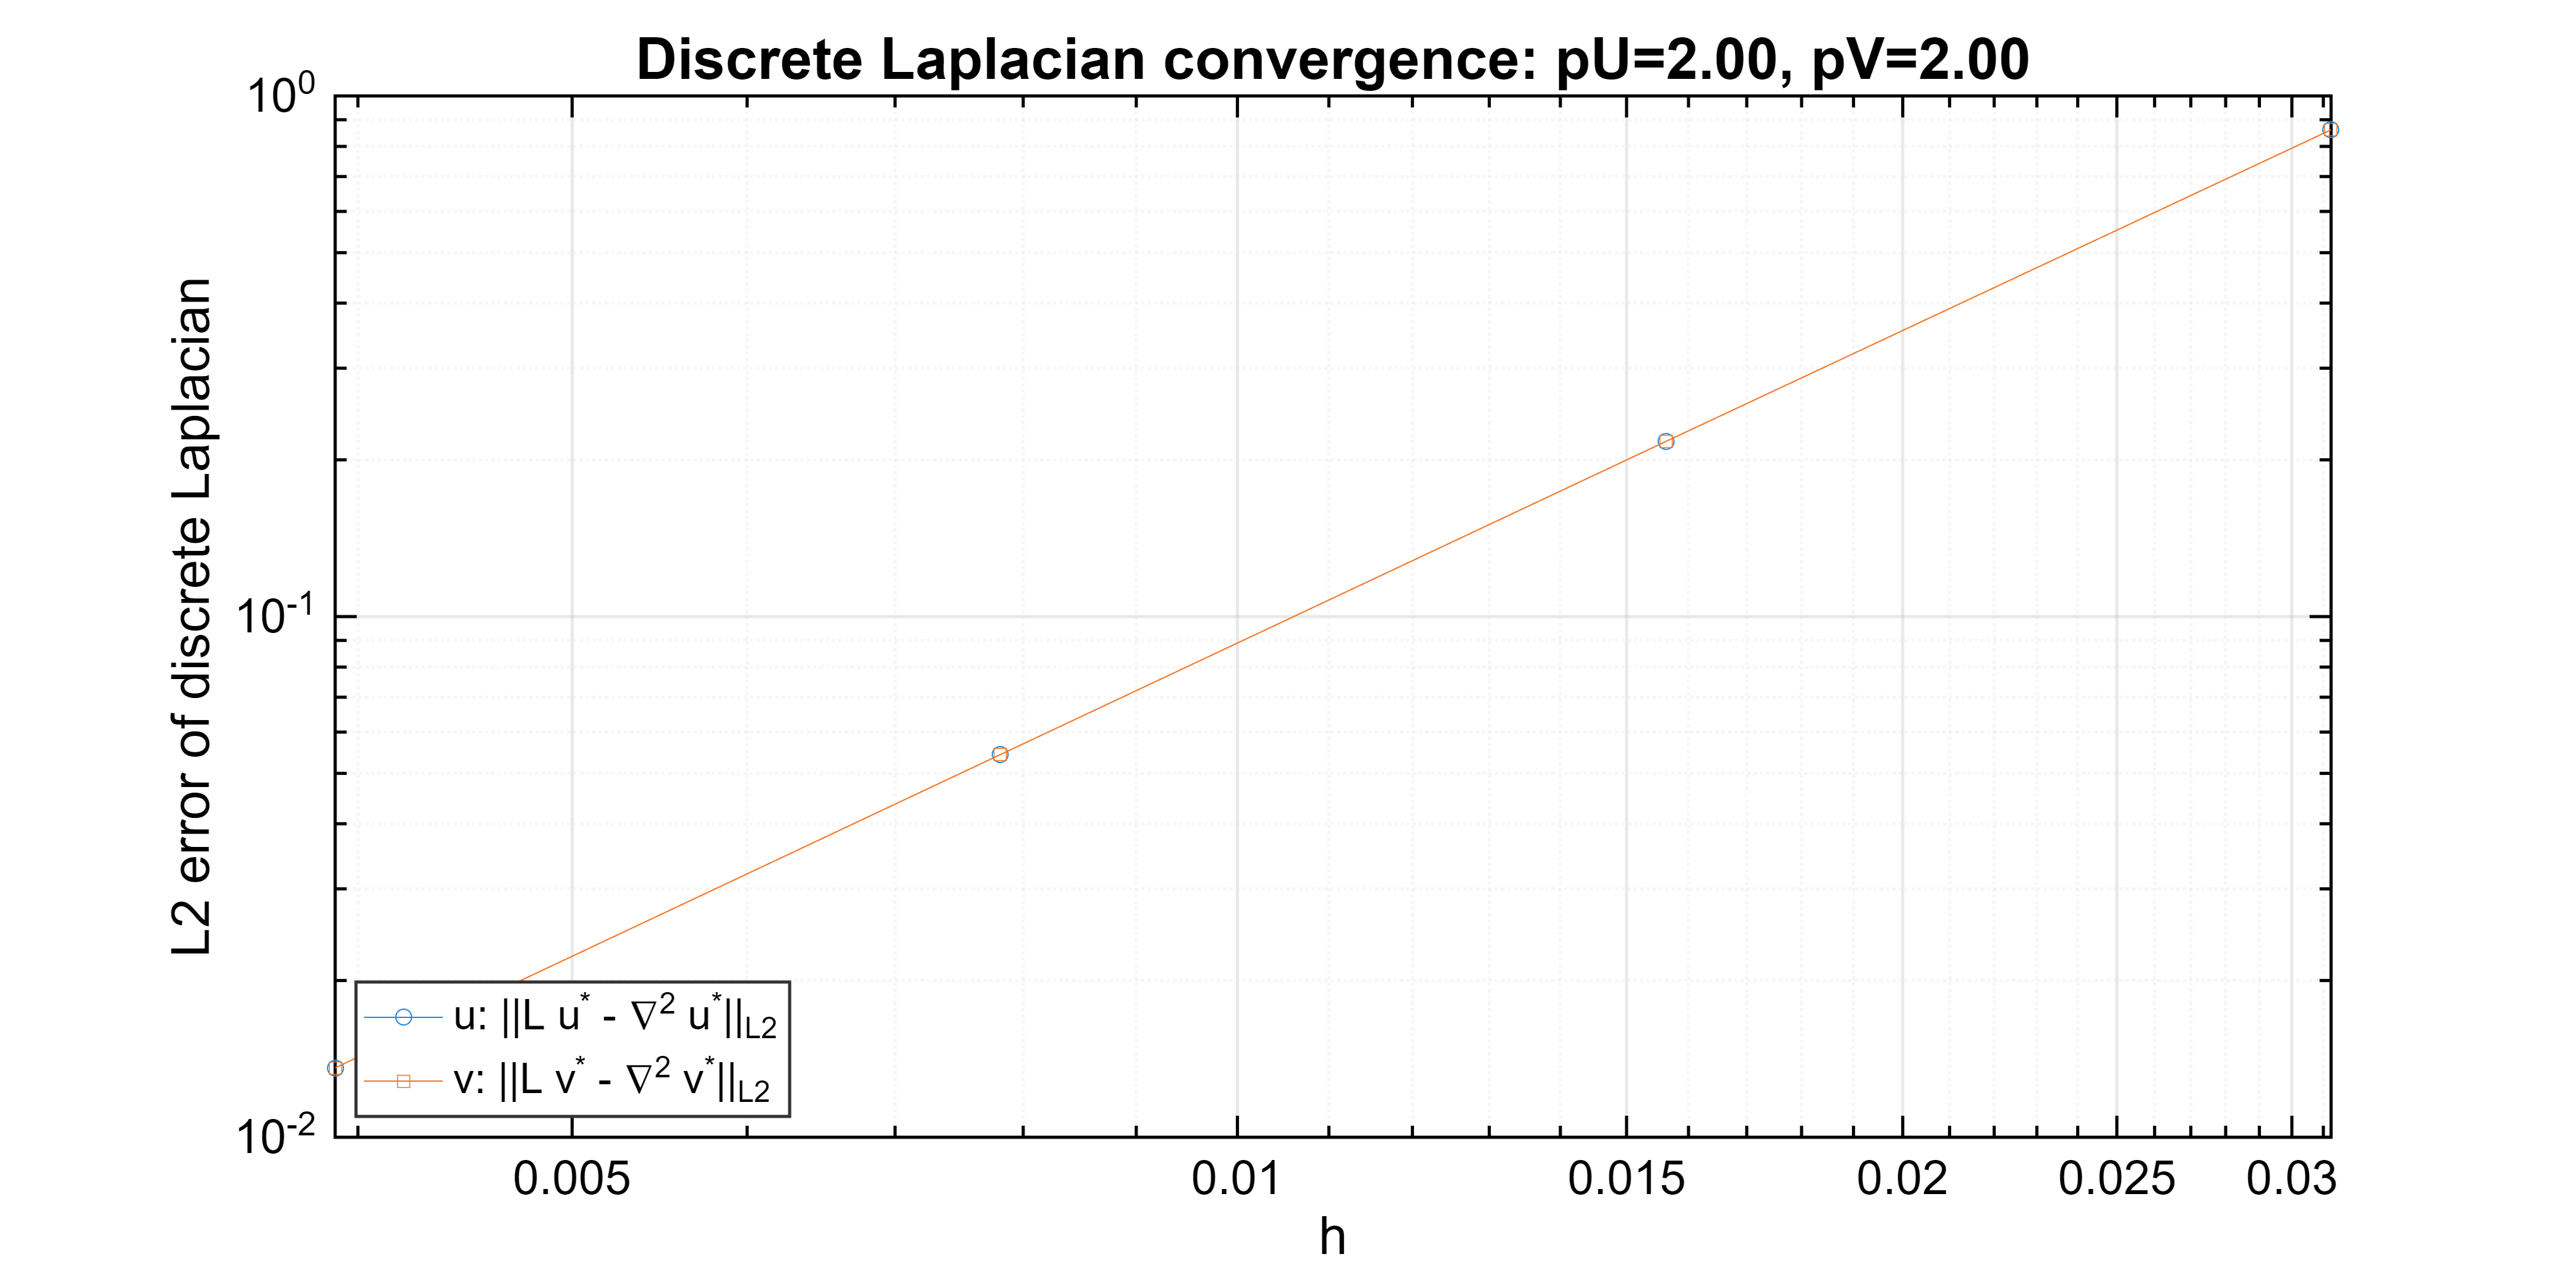
\includegraphics[width=0.82\textwidth]{figures/verification/mms_operator_convergence.png}
\caption{Log--log convergence plot for the discrete Laplacian MMS test.}
\label{fig:mms_operator_convergence}
\end{figure}

\subsection{Test Case 2: Temporal convergence of the explicit Euler scheme}
\label{sec:verification_testcase_timestep_convergence}

\paragraph{Aim.}
This test case verifies the temporal behavior of the explicit Euler time-integration scheme used in the Gray--Scott solver. Since explicit Euler is theoretically first-order accurate in time, the purpose of the test is to check whether the numerical solution shows the expected first-order convergence under time-step refinement while all spatial discretization settings are kept fixed.

\paragraph{Setup.}
The test is performed for the baseline Gray--Scott configuration on the square domain
\[
\Omega = [0,1)\times[0,1),
\]
using a uniform grid with
\[
N_x = N_y = 128.
\]
The model parameters are taken from \texttt{defaultParams()}:
\[
D_u = 2\times 10^{-5}, \qquad
D_v = 1\times 10^{-5}, \qquad
F = 0.03, \qquad
k = 0.06.
\]
Periodic boundary conditions are used on all sides. The final simulation time is
\[
T = 50.
\]

The initial condition is the standard baseline initialization used in the project: the field \(U\) is initialized close to \(1\), the field \(V\) close to \(0\), and a centered \(10\times 10\) square patch is imposed with
\[
U = 0.50, \qquad V = 0.25,
\]
followed by a small random perturbation with amplitude \(\texttt{icPerturb}=0.02\). In order to make the comparison reproducible, the random number generator is reset with the same seed before all runs, so that each simulation starts from exactly the same initial state.

The same problem is then solved three times with the matrix-based diffusion operator and with three different time-step sizes:
\[
\Delta t \in \{0.2,\;0.1,\;0.05\}.
\]
At the final time \(T\), the \(v\)-field of the three runs is compared. Since no exact time-dependent reference solution is used in this test, a self-convergence approach is applied through the successive differences
\[
d_{12} = \|v_{\Delta t} - v_{\Delta t/2}\|,
\qquad
d_{24} = \|v_{\Delta t/2} - v_{\Delta t/4}\|.
\]
These differences are evaluated in both the discrete \(L^2\)-norm and the discrete \(L^\infty\)-norm.

\paragraph{How to run the test case.}
From the project \texttt{tests} folder, run:
\begin{verbatim}
r = test_timestep_convergence();
\end{verbatim}

The test prints the measured successive differences and observed orders to the MATLAB command window and saves the generated figure in the local output folder of
\begin{verbatim}
tests/test_case_02_timestep_convergence/
\end{verbatim}

\paragraph{Expected result.}
For a first-order time-integration method, the temporal discretization error behaves as
\[
e(\Delta t) = C\,\Delta t + \mathcal{O}(\Delta t^2).
\]
Therefore, in the asymptotic regime, the successive-difference indicators are also expected to scale linearly with \(\Delta t\). In particular, halving the time step should approximately halve the difference, so that
\[
\frac{d_{12}}{d_{24}} \approx 2.
\]
The observed order estimate
\[
p = \frac{\log(d_{12}/d_{24})}{\log 2}
\]
should therefore be close to \(1\). In addition, the finer-step difference \(d_{24}\) should be smaller than the coarser-step difference \(d_{12}\).

\paragraph{Obtained result.}
The measured results are listed in Table~\ref{tab:timestep_convergence_data}, and the \(L^2\)-based refinement plot is shown in Fig.~\ref{fig:timestep_convergence}. The numerical results are
\[
d_{12}^{L^2} = 3.706\times 10^{-5}, \qquad
d_{24}^{L^2} = 1.851\times 10^{-5}, \qquad
p_{L^2} = 1.001,
\]
and
\[
d_{12}^{L^\infty} = 5.798\times 10^{-4}, \qquad
d_{24}^{L^\infty} = 2.891\times 10^{-4}, \qquad
p_{L^\infty} = 1.004.
\]

\begin{table}[htbp]
\centering
\caption{Measured successive differences and observed orders for the explicit Euler time-step refinement test.}
\label{tab:timestep_convergence_data}
\begin{tabular}{|c|c|c|c|}
\hline
Norm & \(d_{12}\) & \(d_{24}\) & Observed order \(p\) \\
\hline
\(L^2\)      & \(3.706\times 10^{-5}\) & \(1.851\times 10^{-5}\) & 1.001 \\
\(L^\infty\) & \(5.798\times 10^{-4}\) & \(2.891\times 10^{-4}\) & 1.004 \\
\hline
\end{tabular}
\end{table}

The finer-step difference is smaller than the coarser-step difference in both norms, as expected:
\[
d_{24}^{L^2} < d_{12}^{L^2},
\qquad
d_{24}^{L^\infty} < d_{12}^{L^\infty}.
\]
Moreover, the ratio between successive differences is essentially \(2\), which yields an observed order of approximately \(1\) in both norms. This is in excellent agreement with the theoretical first-order accuracy of the explicit Euler method.

Therefore, the test confirms that the implemented time-integration scheme behaves correctly under time-step refinement and that the solver is operating in the expected temporal convergence regime for this problem configuration.

\begin{figure}[htbp]
\centering
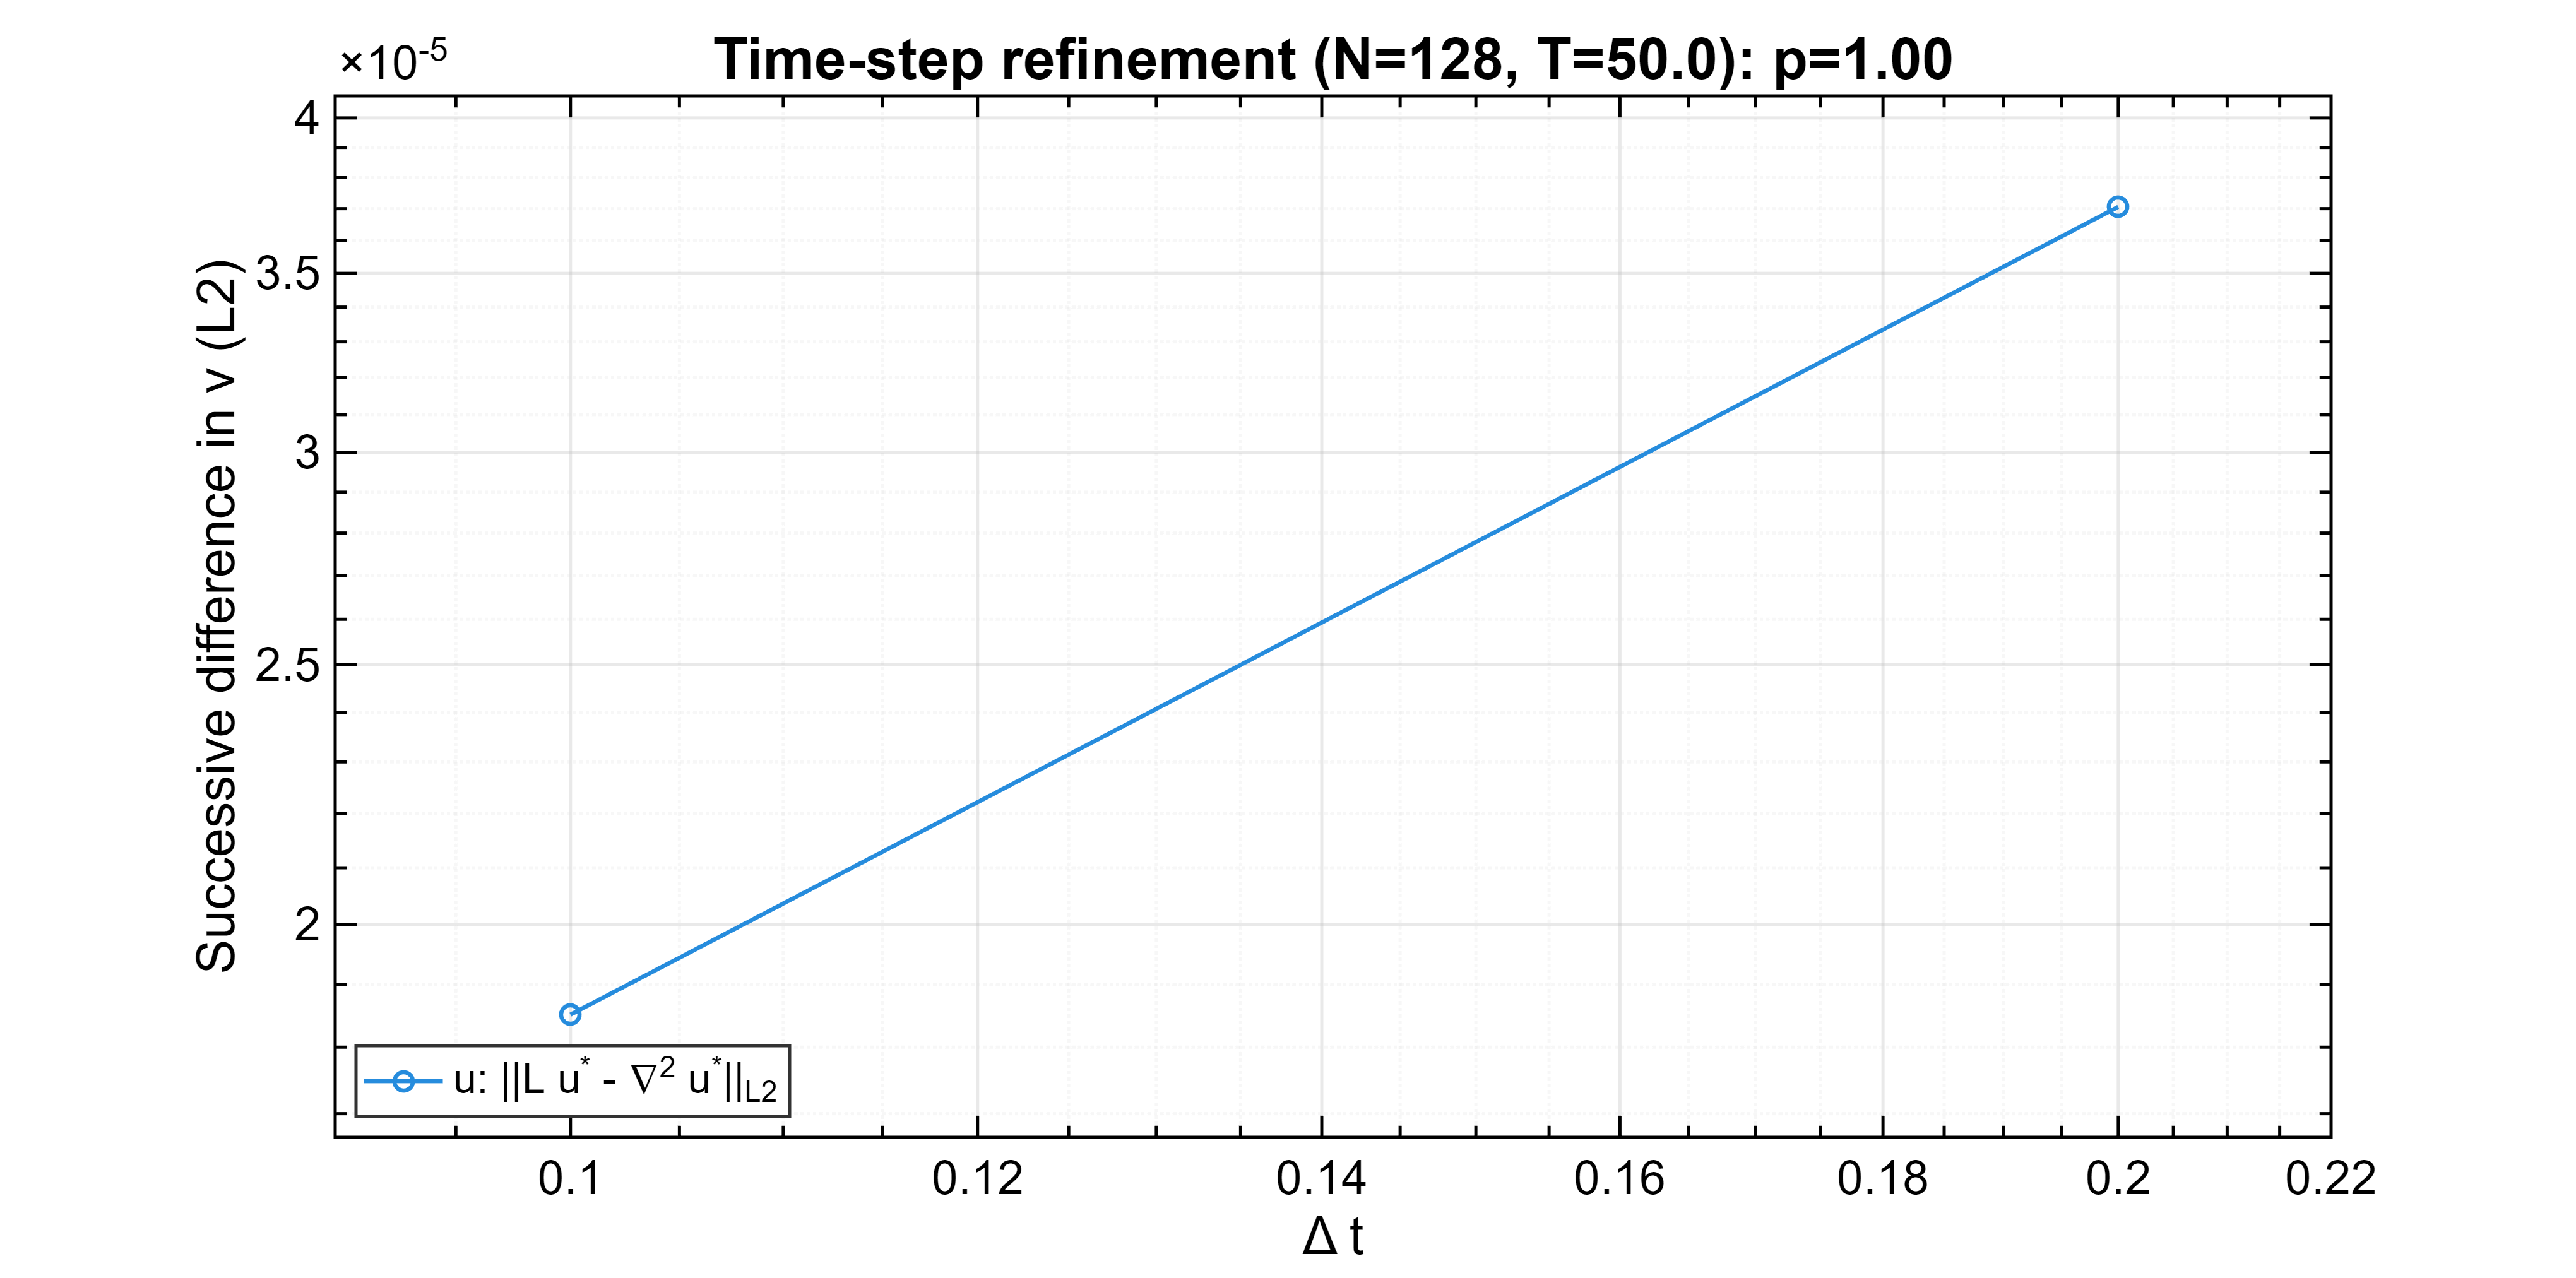
\includegraphics[width=0.82\textwidth]{figures/verification/timestep_convergence.png}
\caption{Time-step refinement test for the explicit Euler scheme. The plot shows the \(L^2\)-based successive differences of the \(v\)-field for \(\Delta t=0.2\) and \(\Delta t=0.1\), indicating first-order temporal convergence.}
\label{fig:timestep_convergence}
\end{figure}


\subsection{Test Case 3: Verification of boundary-condition enforcement}
\label{sec:verification_testcase_boundary_conditions}

\paragraph{Aim.}
This test case verifies that the implemented boundary-condition treatment is applied correctly and robustly in the Gray--Scott solver. Since support for non-periodic boundaries is an explicit feature of the project, it is important to check not only that Dirichlet and Neumann conditions are imposed correctly at the boundary nodes, but also that this enforcement remains stable during time integration and is consistent across all implemented diffusion modes.

\paragraph{Setup.}
The test is performed on the square domain
\[
\Omega = [0,1)\times[0,1)
\]
using a uniform grid with
\[
N_x=N_y=64.
\]
The time step is
\[
\Delta t = 0.25,
\]
and the test is repeated for all three diffusion implementations:
\[
\texttt{matrix}, \qquad \texttt{stencil}, \qquad \texttt{full}.
\]

The verification script combines three sub-checks within one test case.

\medskip
\noindent
\textbf{(1) Dirichlet constant enforcement.}
A smooth nontrivial initial field is prescribed for both species,
\[
U_0(x,y)=0.80+0.10\sin(2\pi x)\cos(2\pi y),
\]
\[
V_0(x,y)=0.20+0.05\cos(2\pi x)\sin(2\pi y),
\]
and a constant Dirichlet condition is imposed on the left boundary:
\[
u = 0.123, \qquad v = 0.456.
\]
The other three boundaries remain periodic. The simulation is advanced for 20 time steps, and after each step the maximum deviation of the left boundary values from the prescribed constants is recorded.

\medskip
\noindent
\textbf{(2) Neumann derivative consistency.}
The same smooth initial fields are used again, but now a constant Neumann condition is prescribed on the left boundary:
\[
\frac{\partial u}{\partial n}=1.0, \qquad \frac{\partial v}{\partial n}=-2.0.
\]
The other boundaries remain periodic. The run is again advanced for 20 time steps. After each step, the normal derivative at the left boundary is approximated by the discrete one-sided difference
\[
\frac{U(:,2)-U(:,1)}{h_x}, \qquad \frac{V(:,2)-V(:,1)}{h_x},
\]
and the maximum deviation from the prescribed derivative values is recorded.

\medskip
\noindent
\textbf{(3) Mixed boundary-condition robustness test.}
A more demanding long-time test is then performed with a strongly mismatched initial state,
\[
U_0 = 0.95, \qquad V_0 = 0.05
\]
throughout the interior, while the following boundary conditions are imposed:
\[
u=0.2,\quad v=0.4 \qquad \text{on the left boundary (Dirichlet)},
\]
\[
\frac{\partial u}{\partial n}=0,\quad \frac{\partial v}{\partial n}=0
\qquad \text{on the right boundary (Neumann)},
\]
with periodic boundaries at the top and bottom. This case is run for 400 time steps, corresponding to
\[
T = 100.
\]
During the run, the maximum boundary errors are tracked for both the Dirichlet and Neumann sides. In addition, an interior monitoring column is monitored in order to confirm that the solution evolves nontrivially in the interior and that the test is not merely a static boundary overwrite. The script also checks that no \texttt{NaN} or \texttt{Inf} values occur.

\paragraph{How to run the test case.}
From the project \texttt{tests} folder, run:
\begin{verbatim}
r = test_boundary_conditions();
\end{verbatim}

The test prints the maximum boundary errors for all three diffusion modes in the MATLAB command window.

\paragraph{Expected result.}
For the Dirichlet sub-test, the prescribed boundary values should be enforced exactly at every time step, up to machine precision. Therefore, the maximum boundary error should be essentially zero.

For the Neumann sub-test, the discrete boundary gradient should match the prescribed normal derivative. Since the condition is imposed directly in the discrete formulation, the resulting error should again be at the level of roundoff.

For the mixed long-time test, the left Dirichlet boundary should remain fixed at its prescribed values and the right Neumann boundary should remain zero-flux throughout the simulation. At the same time, the interior should evolve measurably away from the initial state. Thus, the expected result is:
\begin{itemize}
    \item boundary errors at or near machine precision,
    \item no \texttt{NaN} or \texttt{Inf} values,
    \item nonzero interior change,
    \item and identical qualitative behavior for \texttt{matrix}, \texttt{stencil}, and \texttt{full} modes.
\end{itemize}

\paragraph{Obtained result.}
All checks passed for all three diffusion modes. The returned test result was
\[
\texttt{pass} = 1,
\]
and the script reported that the quantitative Dirichlet, Neumann, and mixed boundary-condition checks passed for \texttt{matrix}, \texttt{stencil}, and \texttt{full} modes.

The measured results are summarized separately in Tables~\ref{tab:bc_dirichlet_verification}, \ref{tab:bc_neumann_verification}, and \ref{tab:bc_mixed_verification}. For the Dirichlet test, the maximum boundary error was exactly zero for both \(u\) and \(v\) in all three modes over 20 steps. For the Neumann test, the maximum error was zero for \(u\) and
\[
3.553\times 10^{-15}
\]
for \(v\), which is at the level of machine precision and therefore consistent with exact discrete enforcement up to floating-point roundoff.

In the mixed 400-step test, the maximum Dirichlet and Neumann boundary errors remained zero for both species in all three diffusion modes. At the same time, the interior change values changed by
\[
2.992\times 10^{-2} \quad \text{for } u,
\qquad
4.982\times 10^{-2} \quad \text{for } v,
\]
which confirms that the solution evolved nontrivially in the interior while the imposed boundary conditions remained exactly enforced.

The fact that the reported errors are identical for \texttt{matrix}, \texttt{stencil}, and \texttt{full} is a strong indication that the boundary-condition handling is implemented consistently across all diffusion formulations.

\begin{table}[htbp]
\centering
\caption{Dirichlet boundary-condition verification results for all diffusion modes.}
\label{tab:bc_dirichlet_verification}
\begin{tabular}{|c|c|c|}
\hline
Mode & maxErr \(u\) & maxErr \(v\) \\
\hline
\texttt{matrix}  & \(0.000\times 10^{0}\) & \(0.000\times 10^{0}\) \\
\texttt{stencil} & \(0.000\times 10^{0}\) & \(0.000\times 10^{0}\) \\
\texttt{full}    & \(0.000\times 10^{0}\) & \(0.000\times 10^{0}\) \\
\hline
\end{tabular}
\end{table}

\begin{table}[htbp]
\centering
\caption{Neumann boundary-condition verification results for all diffusion modes.}
\label{tab:bc_neumann_verification}
\begin{tabular}{|c|c|c|}
\hline
Mode & maxErr \(u\) & maxErr \(v\) \\
\hline
\texttt{matrix}  & \(0.000\times 10^{0}\) & \(3.553\times 10^{-15}\) \\
\texttt{stencil} & \(0.000\times 10^{0}\) & \(3.553\times 10^{-15}\) \\
\texttt{full}    & \(0.000\times 10^{0}\) & \(3.553\times 10^{-15}\) \\
\hline
\end{tabular}
\end{table}

\begin{table}[htbp]
\centering
\small
\setlength{\tabcolsep}{4pt}
\renewcommand{\arraystretch}{1.15}
\caption{Mixed boundary-condition robustness results for all diffusion modes after 400 steps.}
\label{tab:bc_mixed_verification}
\begin{tabular}{|c|c|c|c|c|c|c|}
\hline
Mode
& \shortstack{maxDir\\\(u\)}
& \shortstack{maxDir\\\(v\)}
& \shortstack{maxNeu\\\(u\)}
& \shortstack{maxNeu\\\(v\)}
& \shortstack{interior\\change \(\Delta u\)}
& \shortstack{interior\\change \(\Delta v\)} \\
\hline
\texttt{matrix}  & \(0.000\times 10^{0}\) & \(0.000\times 10^{0}\) & \(0.000\times 10^{0}\) & \(0.000\times 10^{0}\) & \(2.992\times 10^{-2}\) & \(4.982\times 10^{-2}\) \\
\texttt{stencil} & \(0.000\times 10^{0}\) & \(0.000\times 10^{0}\) & \(0.000\times 10^{0}\) & \(0.000\times 10^{0}\) & \(2.992\times 10^{-2}\) & \(4.982\times 10^{-2}\) \\
\texttt{full}    & \(0.000\times 10^{0}\) & \(0.000\times 10^{0}\) & \(0.000\times 10^{0}\) & \(0.000\times 10^{0}\) & \(2.992\times 10^{-2}\) & \(4.982\times 10^{-2}\) \\
\hline
\end{tabular}
\end{table}

Overall, this test case confirms that the boundary-condition treatment is not only mathematically correct at the discrete level, but also numerically robust during time stepping and consistent across all solver variants used in the project.


\subsection{Test Case 4: Matrix--stencil equivalence of the diffusion operator}
\label{sec:verification_testcase_laplacian_equivalence}

\paragraph{Aim.}
This test case verifies that the two implemented diffusion-operator realizations, namely the sparse matrix formulation and the matrix-free stencil formulation, produce the same numerical result when applied to the same discrete field. Since both implementations are intended to represent the same five-point finite-difference Laplacian on a periodic grid, this test is an important consistency check at the operator level.

\paragraph{Setup.}
The test compares the output of the sparse matrix Laplacian assembled by \texttt{buildLaplacian2D} with the output of the matrix-free stencil operator evaluated by \texttt{applyLaplacianStencil}. The comparison is carried out for periodic connectivity only, because physical boundary conditions such as Dirichlet and Neumann are imposed separately after each time step and are therefore not part of this operator-equivalence test.

Three different grid sizes are used in order to detect possible indexing, reshaping, or dimension-ordering mistakes:
\[
32\times 32,\qquad 64\times 48,\qquad 128\times 128.
\]
For each grid, three independent random trials are performed. In each trial, a random discrete field \(u\) is generated, and the following two operator evaluations are computed:
\[
a = Lu,
\qquad
b = \mathcal{S}(u),
\]
where \(L\) denotes the sparse matrix Laplacian and \(\mathcal{S}\) denotes the stencil-based Laplacian application.

The difference between the two results is measured using:
\[
\text{relative error} = \frac{\|a-b\|_2}{\max(1,\|a\|_2)},
\]
and
\[
\text{maximum absolute difference} = \max_i |a_i-b_i|.
\]

The tolerances used by the test are
\[
\texttt{relTol} = 10^{-12},
\qquad
\texttt{absTol} = 10^{-10}.
\]

\paragraph{How to run the test case.}
From the project \texttt{tests} folder, run:
\begin{verbatim}
r = test_laplacian_stencil_equivalence();
\end{verbatim}

The test prints the relative and absolute differences for each grid and trial and reports the worst observed case.

\paragraph{Expected result.}
Both implementations represent the same discrete Laplacian operator. Therefore, for the same input vector \(u\), their outputs should agree up to floating-point roundoff. As a result, the relative error should be extremely small, and the maximum absolute difference should remain below the prescribed numerical tolerances. In particular, all trials should pass with margins far below
\[
10^{-12}\quad \text{(relative)}
\qquad\text{and}\qquad
10^{-10}\quad \text{(absolute)}.
\]

\paragraph{Obtained result.}
All nine test cases passed successfully, and the returned result was
\[
\texttt{pass} = 1.
\]
The measured values are listed in Table~\ref{tab:matrix_stencil_operator_equivalence}. The relative errors were consistently on the order of \(10^{-16}\), which is close to machine precision. The largest observed relative error was
\[
1.249\times 10^{-16}
\]
for the \(64\times 48\) grid in trial 2. The largest observed maximum absolute difference was
\[
5.821\times 10^{-11}
\]
for the \(128\times 128\) grid in trial 1.

These worst-case values are still safely below the prescribed tolerances:
\[
1.249\times 10^{-16} \ll 10^{-12},
\qquad
5.821\times 10^{-11} < 10^{-10}.
\]
The slightly larger absolute differences on the finest grid are expected because larger systems may accumulate somewhat more floating-point roundoff, but the differences remain numerically negligible.

Therefore, the test confirms that the matrix-based and stencil-based diffusion operators are equivalent to machine precision and can be regarded as two consistent implementations of the same finite-difference Laplacian.

\begin{table}[htbp]
\centering
\caption{Matrix--stencil operator equivalence results for all tested grids and trials.}
\label{tab:matrix_stencil_operator_equivalence}
\begin{tabular}{|c|c|c|c|}
\hline
Grid & Trial & Relative error & Max absolute difference \\
\hline
\(32\times 32\)   & 1 & \(1.145\times 10^{-16}\) & \(3.638\times 10^{-12}\) \\
\(32\times 32\)   & 2 & \(1.127\times 10^{-16}\) & \(1.819\times 10^{-12}\) \\
\(32\times 32\)   & 3 & \(1.132\times 10^{-16}\) & \(1.819\times 10^{-12}\) \\
\(64\times 48\)   & 1 & \(1.211\times 10^{-16}\) & \(7.276\times 10^{-12}\) \\
\(64\times 48\)   & 2 & \(1.249\times 10^{-16}\) & \(1.455\times 10^{-11}\) \\
\(64\times 48\)   & 3 & \(1.181\times 10^{-16}\) & \(7.276\times 10^{-12}\) \\
\(128\times 128\) & 1 & \(1.131\times 10^{-16}\) & \(5.821\times 10^{-11}\) \\
\(128\times 128\) & 2 & \(1.132\times 10^{-16}\) & \(5.821\times 10^{-11}\) \\
\(128\times 128\) & 3 & \(1.118\times 10^{-16}\) & \(5.821\times 10^{-11}\) \\
\hline
\end{tabular}
\end{table}


\subsection{Test Case 5: End-to-end equivalence of matrix and stencil solver modes}
\label{sec:verification_testcase_solver_equivalence}

\paragraph{Aim.}
This test case verifies that the matrix-based and stencil-based diffusion modes are equivalent at the level of the full Gray--Scott simulation, not only at the isolated operator level. In contrast to the previous operator-equivalence test, this case checks the complete solver workflow, including model initialization, time stepping, reaction evaluation, diffusion application, and state updates. Its purpose is to confirm that both solver modes produce the same final numerical solution when they are run with identical settings.

\paragraph{Setup.}
The test uses the full \texttt{GrayScottModel} class on the square periodic domain
\[
\Omega = [0,1)\times[0,1),
\]
with a uniform grid
\[
N_x = N_y = 128.
\]
The standard project parameters from \texttt{defaultParams()} are used:
\[
D_u = 2\times 10^{-5}, \qquad
D_v = 1\times 10^{-5}, \qquad
F = 0.03, \qquad
k = 0.06.
\]
The time step is
\[
\Delta t = 0.2,
\]
and the final simulation time is
\[
T = 5.
\]

Two runs are then carried out:

\begin{itemize}
    \item a baseline run with \texttt{diffusionMode = "matrix"},
    \item a comparison run with \texttt{diffusionMode = "stencil"}.
\end{itemize}

To ensure that both runs start from exactly the same initial condition, the random number generator is reset to the same seed before each run. The same grid and the same model parameters are used in both cases. After both simulations reach the final time \(T\), the final states are compared componentwise.

Let \(u_A, v_A\) denote the final matrix-mode solution and \(u_B, v_B\) the final stencil-mode solution. The test evaluates the differences
\[
d_u = u_A - u_B, \qquad d_v = v_A - v_B,
\]
and computes both relative and maximum absolute differences:
\[
\mathrm{rel}_u = \frac{\|d_u\|_2}{\max(1,\|u_A\|_2)}, \qquad
\mathrm{rel}_v = \frac{\|d_v\|_2}{\max(1,\|v_A\|_2)},
\]
\[
\mathrm{max}_u = \max_i |d_{u,i}|, \qquad
\mathrm{max}_v = \max_i |d_{v,i}|.
\]

The tolerances used by the test are
\[
\texttt{relTol} = 10^{-10}, \qquad
\texttt{absTol} = 10^{-9}.
\]

\paragraph{How to run the test case.}
From the project \texttt{tests} folder, run:
\begin{verbatim}
r = test_matrix_stencil_endtoend_equivalence();
\end{verbatim}

The test prints the measured relative and maximum absolute differences in the MATLAB command window.

\paragraph{Expected result.}
If the matrix-based and stencil-based diffusion modes are truly equivalent implementations of the same numerical method, then the complete Gray--Scott runs should produce the same final solution up to floating-point roundoff. Therefore, the relative differences in both \(u\) and \(v\) should be extremely small, and the maximum absolute differences should remain far below the prescribed tolerances. In particular, both solution components should satisfy
\[
\mathrm{rel}_u < 10^{-10}, \qquad \mathrm{rel}_v < 10^{-10},
\]
and
\[
\mathrm{max}_u < 10^{-9}, \qquad \mathrm{max}_v < 10^{-9}.
\]

\paragraph{Obtained result.}
The test passed successfully, and the returned result was
\[
\texttt{pass} = 1.
\]
The measured final-state differences are summarized in Table~\ref{tab:matrix_stencil_endtoend_equivalence}.

\begin{table}[htbp]
\centering
\caption{End-to-end comparison between matrix and stencil solver modes at final time \(T=5\).}
\label{tab:matrix_stencil_endtoend_equivalence}
\begin{tabular}{|c|c|}
\hline
Quantity & Measured value \\
\hline
\(\mathrm{rel}_u\) & \(8.903\times 10^{-17}\) \\
\(\mathrm{rel}_v\) & \(9.927\times 10^{-17}\) \\
\(\mathrm{max}_u\) & \(4.441\times 10^{-16}\) \\
\(\mathrm{max}_v\) & \(5.551\times 10^{-17}\) \\
\hline
\end{tabular}
\end{table}

All reported differences are many orders of magnitude smaller than the specified tolerances:
\[
8.903\times 10^{-17} \ll 10^{-10}, \qquad
9.927\times 10^{-17} \ll 10^{-10},
\]
\[
4.441\times 10^{-16} \ll 10^{-9}, \qquad
5.551\times 10^{-17} \ll 10^{-9}.
\]
Thus, the final solutions produced by the two solver modes are numerically indistinguishable up to machine precision.

This result shows that the stencil-based and matrix-based implementations remain consistent not only when applying the Laplacian to a test vector, but also when embedded in the full Gray--Scott time integration process.


\subsection{Test Case 6: GUI and non-GUI consistency}
\label{sec:verification_testcase_gui_consistency}

\paragraph{Aim.}
This test case verifies that the graphical user interface does not alter the numerical model and that a simulation executed through the GUI reproduces exactly the same numerical results as the corresponding non-GUI workflow. The purpose is to check consistency at the interface level, i.e.\ to confirm that the GUI acts only as a control and visualization layer and does not introduce unintended changes in parameters, initialization, or solver behavior.

\paragraph{Setup.}
The consistency check is carried out in three stages. First, a non-GUI reference run is generated using the same parameter set as the GUI startup configuration. Second, the GUI is launched with its current shipped default setup and a dedicated helper script advances the GUI-owned model for the exact number of required time steps. Third, the saved non-GUI and GUI results are compared quantitatively.

For the run documented here, the GUI startup configuration was:
\[
\texttt{preset}=\texttt{pearson}, \qquad
\texttt{diffusionMode}=\texttt{stencil},
\]
with periodic boundary conditions on all sides. The computational grid was
\[
N_x = N_y = 256,
\]
the time step was
\[
\Delta t = 0.5,
\]
and the final simulation time was
\[
T = 500.
\]
Therefore, the total number of time steps was
\[
n_{\text{steps}} = \frac{T}{\Delta t} = \frac{500}{0.5} = 1000.
\]
A midpoint snapshot was stored at
\[
k_{\text{snap}} = 500.
\]

The comparison includes both the midpoint snapshot and the final state for the two species \(u\) and \(v\). For each compared field, the following quantities are evaluated:
\[
\mathrm{relL2} = \frac{\|w_{\mathrm{GUI}} - w_{\mathrm{ref}}\|_2}{\max(1,\|w_{\mathrm{ref}}\|_2)},
\qquad
\mathrm{maxAbs} = \max_i |w_{\mathrm{GUI},i} - w_{\mathrm{ref},i}|.
\]
The tolerances used by the comparison script are
\[
\texttt{tol\_relL2} = 10^{-12},
\qquad
\texttt{tol\_maxAbs} = 10^{-12}.
\]

The relevant scripts are:
\begin{verbatim}
run_nongui_reference_dump.m
run_gui_consistency_dump.m
compare_gui_nongui.m
\end{verbatim}

All three files are located in:
\begin{verbatim}
tests/test_case_06_gui_nongui_consistency/
\end{verbatim}

\paragraph{How to run the test case.}
Run the workflow either from the project root or from
\texttt{tests/test\_case\_06\_gui\_nongui\_consistency}. Make sure that the project paths are available. Then execute:
\begin{verbatim}
ref = run_nongui_reference_dump();
gui = run_gui_consistency_dump();
T   = compare_gui_nongui(ref.refFile, gui.guiFile);
\end{verbatim}

The first two helper scripts save their generated \texttt{.mat} files in the local output folder of
\texttt{tests/test\_case\_06\_gui\_nongui\_consistency/}. The comparison script can read those files directly when their paths are passed explicitly, as shown above. If \texttt{compare\_gui\_nongui()} is called without arguments, it instead searches for comparison input files in the local \texttt{inputs/} folder.

For the documented run, the workflow produced the non-GUI dump, the GUI dump, the comparison CSV file, and the comparison figure in the local output folder
\begin{verbatim}
tests/test_case_06_gui_nongui_consistency/
\end{verbatim}

\paragraph{Expected result.}
If the GUI is consistent with the underlying solver implementation, then the GUI-generated run and the non-GUI reference run should produce identical or numerically indistinguishable data when started from the same configuration. Since this test uses the same model parameters, same grid, same seed, same number of steps, and the same solver configuration, the expected result is that both the midpoint snapshot and the final state match within the very strict tolerances
\[
10^{-12}
\]
for both the relative \(L^2\) difference and the maximum absolute difference.

\paragraph{Obtained result.}
The comparison passed in all four checked cases: snapshot \(u\), snapshot \(v\), final \(u\), and final \(v\). The measured results are summarized in Table~\ref{tab:gui_nongui_consistency}. In every case,
\[
\mathrm{relL2} = 0,
\qquad
\mathrm{maxAbs} = 0,
\]
and the pass flag was \texttt{true}. Therefore, the GUI and non-GUI workflows produced exactly identical saved states for both the midpoint snapshot and the final solution.

\begin{table}[htbp]
\centering
\caption{GUI and non-GUI consistency comparison results.}
\label{tab:gui_nongui_consistency}
\begin{tabular}{|c|c|c|c|c|}
\hline
Stage & Field & relL2 & maxAbs & Pass \\
\hline
snapshot & \(u\) & 0 & 0 & true \\
snapshot & \(v\) & 0 & 0 & true \\
final    & \(u\) & 0 & 0 & true \\
final    & \(v\) & 0 & 0 & true \\
\hline
\end{tabular}
\end{table}

Figure~\ref{fig:gui_nongui_consistency} shows the GUI--non-GUI difference field for the snapshot of \(u\). The plotted field is identically zero, which is fully consistent with the tabulated comparison metrics. The same conclusion applies to the other compared states as well.

Hence, this test confirms that the GUI layer does not modify the mathematical or numerical behavior of the solver. It reproduces the same results as the non-GUI reference workflow exactly for the tested configuration.

\begin{figure}[htbp]
\centering
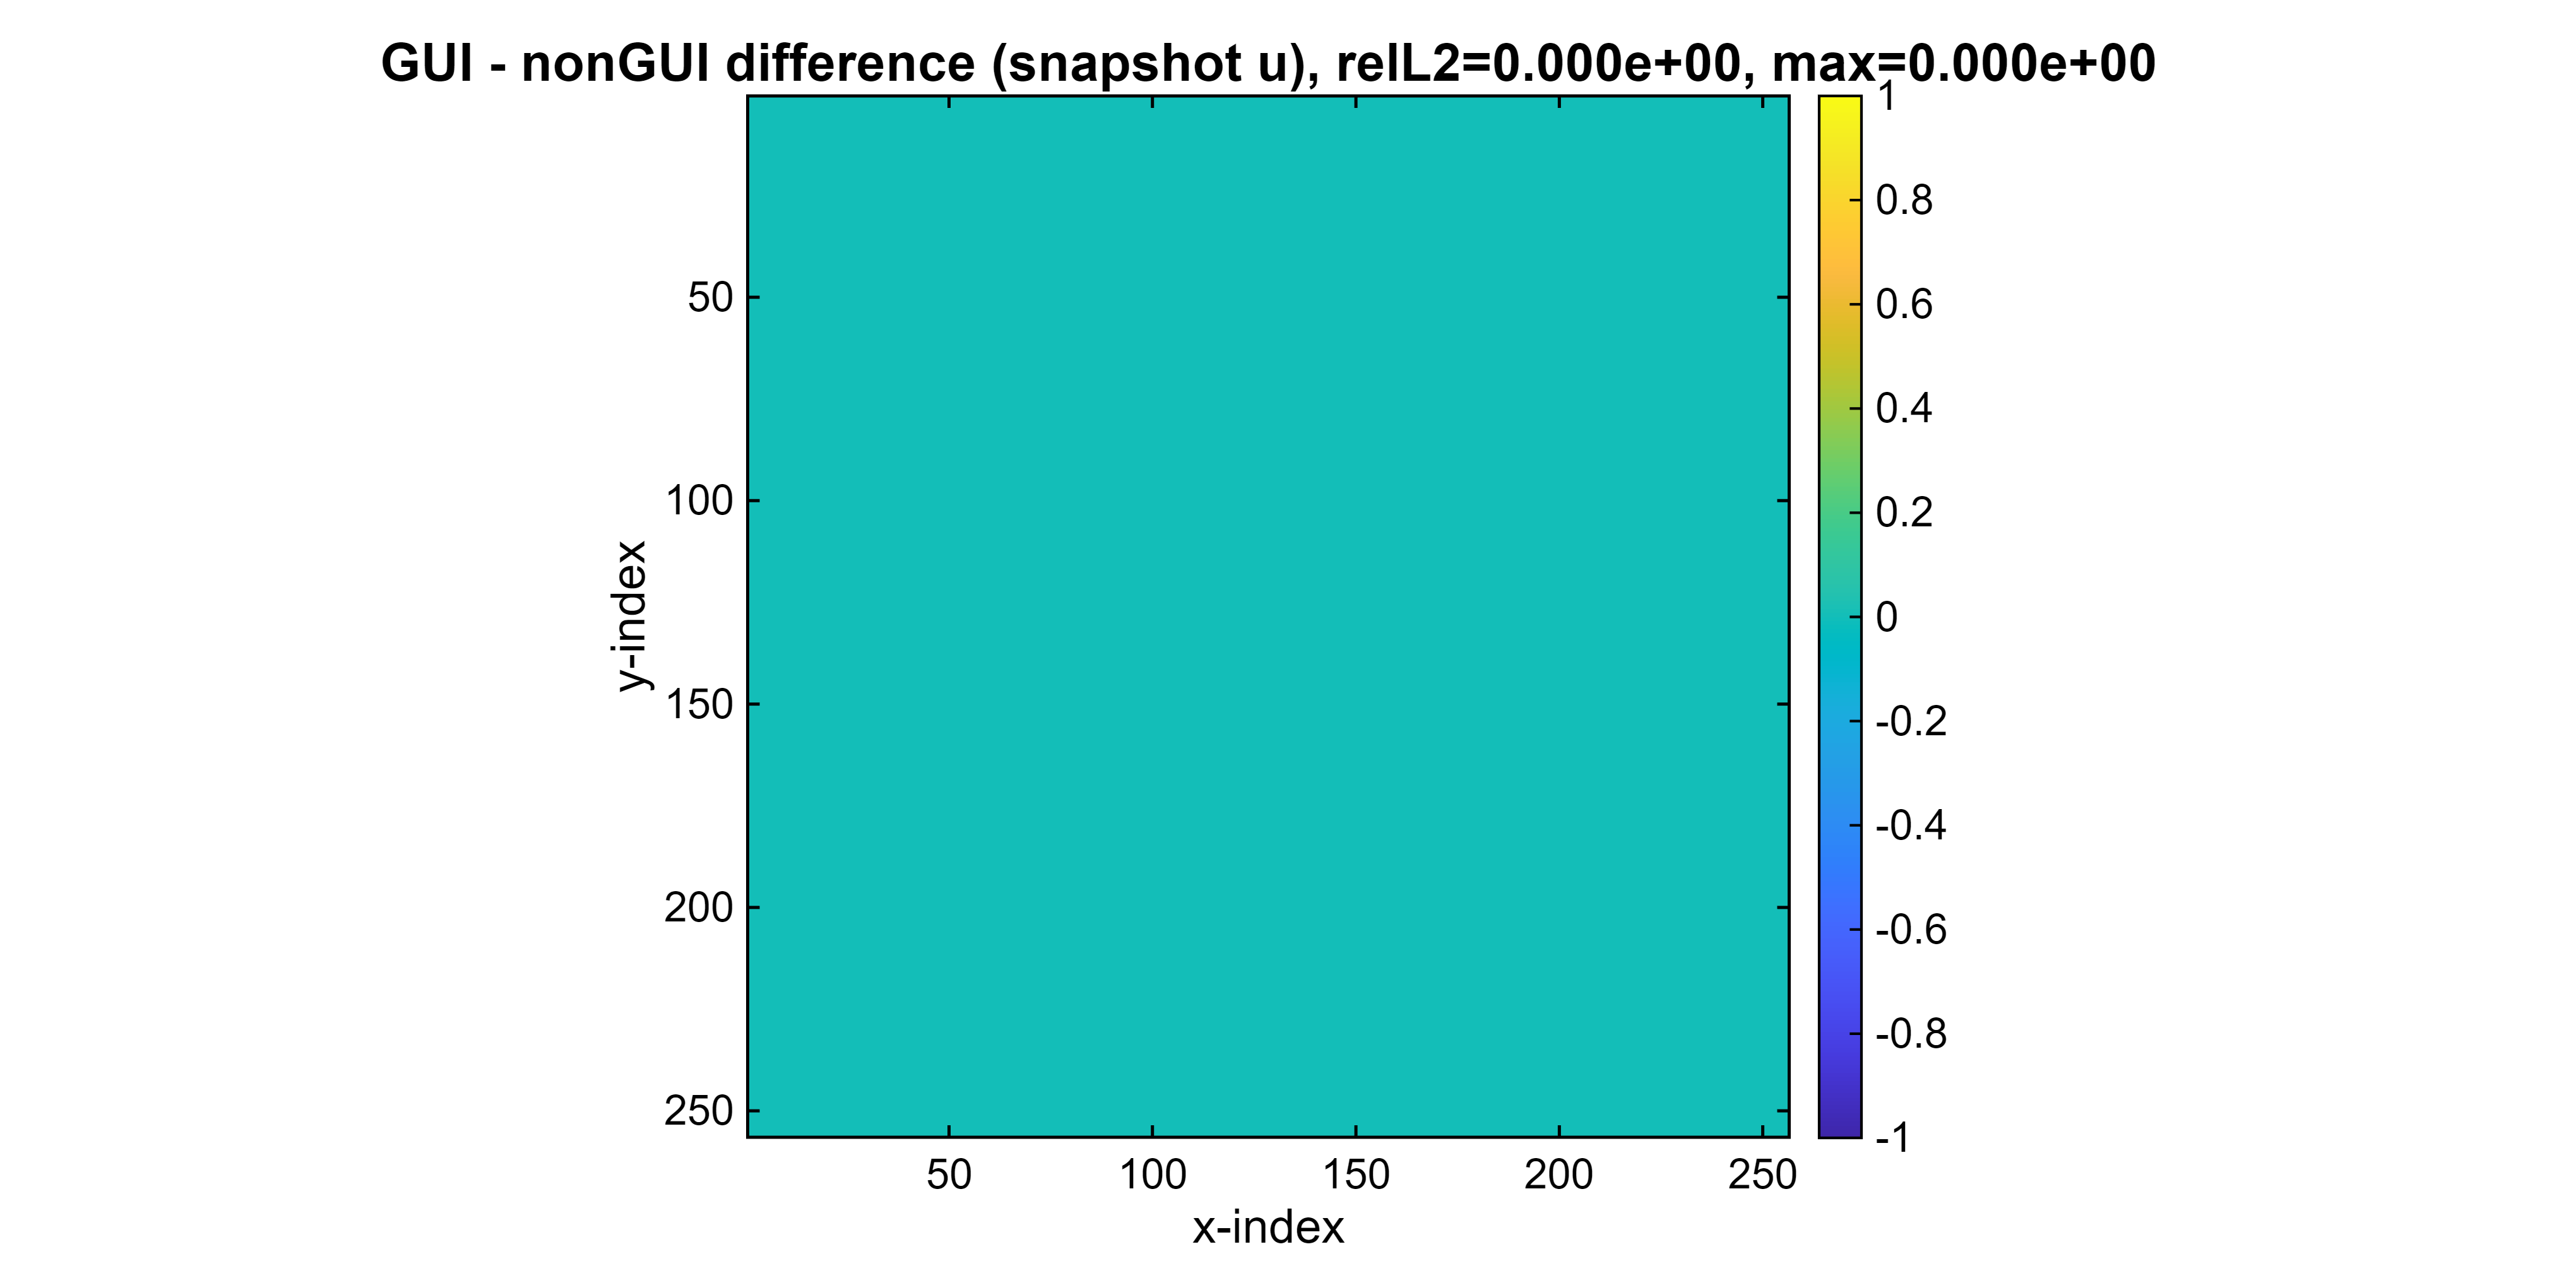
\includegraphics[width=0.78\textwidth]{figures/verification/gui_consistency.png}
\caption{Difference field between GUI and non-GUI results for the snapshot of \(u\). The field is identically zero, confirming exact agreement for the documented run.}
\label{fig:gui_nongui_consistency}
\end{figure}

\subsection{Test Case 7: Gray--Scott grid refinement test}
\label{sec:verification_testcase_grid_refinement}

\paragraph{Aim.}
This test case investigates how the numerical solution of the full nonlinear Gray--Scott system changes under spatial grid refinement. Unlike the manufactured-solution tests, this is not an exact-solution verification test, because no analytical reference solution is available for the pattern-forming nonlinear problem considered here. The goal is therefore more practical: to check whether the computed solution approaches a sufficiently fine-grid reference in a systematic way as the mesh is refined, and whether the observed behavior is consistent with the expected second-order spatial discretization used in the solver.

\paragraph{Initial idea and first difficulty.}
The original idea of this test was straightforward. The Gray--Scott system was solved on a sequence of grids, the finest grid was used as a numerical reference, and the coarser-grid solutions were compared against that reference in the discrete \(L^2\) norm. The time step was scaled as \(\Delta t \sim h^2\) in order to reduce the influence of the first-order explicit Euler time discretization and make the comparison mainly sensitive to spatial effects.

However, the first version of the test did not give the expected result. Although the errors decreased monotonically under refinement, the observed rates remained noticeably below the ideal value \(2\). At first sight, this could suggest that the fully nonlinear Gray--Scott dynamics, especially the phase-sensitive pattern evolution, prevented a clean refinement study. A closer inspection showed that this was only part of the explanation.

\paragraph{Why the first version was not fully reliable.}
The main issue in the original version was that the initialization was not grid-independent. The standard Gray--Scott pattern-seeding setup used in the project is suitable for normal simulations, but it is not ideal for a formal refinement study. In particular, the original initialization contained two features that made the comparison across grids less clean:

\begin{enumerate}
    \item The initial square perturbation was prescribed in a fixed number of grid cells rather than in physical coordinates. As a result, its physical size changed when the grid was refined.
    \item A random perturbation was added independently on each grid. Even with the same random seed, this does not represent the same physical perturbation sampled on different meshes.
\end{enumerate}

Therefore, the different grid levels did not correspond to exactly the same initial-value problem. For a nonlinear pattern-forming PDE such as the Gray--Scott system, even small differences in the initial condition can later produce visible phase shifts, slight pattern displacements, and morphology changes. Consequently, the discrete \(L^2\) difference between two solutions may reflect not only discretization error, but also mismatch in the underlying evolving pattern.

This analysis explained why the original version produced only moderate observed rates even though the error still decreased consistently.

\paragraph{Correction of the test design.}
To make the refinement study meaningful, the test was reformulated so that all grid levels solve the same problem as closely as possible. Two changes were introduced:

\begin{enumerate}
    \item The original grid-dependent seeded pattern was replaced by a smooth Gaussian-type initial condition defined directly in physical coordinates.
    \item The random perturbation was disabled for this test.
\end{enumerate}

With these two changes, every grid represents the same smooth initial state sampled at different resolutions. This removes the main inconsistency of the original setup and makes the subsequent comparison much more suitable for measuring refinement behavior.

In addition, the final simulation time was reduced to
\[
T = 0.2,
\]
instead of using a longer pattern-development time. This makes the test less sensitive to long-time nonlinear phase drift and allows the spatial discretization error to remain the dominant effect.

\paragraph{Final setup used for the reported result.}
The corrected test was carried out for the Gray--Scott model on the periodic square domain
\[
\Omega = [0,1)\times[0,1)
\]
with the baseline parameter set
\[
D_u = 2\times 10^{-5}, \qquad
D_v = 1\times 10^{-5}, \qquad
F = 0.03, \qquad
k = 0.06.
\]
The problem was solved on the sequence of uniform grids
\[
N_x=N_y \in \{64,\,128,\,256,\,512,\,1024,\,2048\}.
\]
The finest grid,
\[
N_x=N_y=2048,
\]
was used as the numerical reference solution. The reference fields were interpolated onto the coarser grids using cubic interpolation before computing the discrete \(L^2\) differences.

The time step was again scaled as
\[
\Delta t \sim h^2,
\]
with
\[
\Delta t = 0.01 \quad \text{for } N=64,
\]
and then reduced by a factor of four whenever the grid spacing was halved. This gives
\[
\Delta t \in \left\{
0.01,\;
0.0025,\;
0.000625,\;
0.00015625,\;
3.90625\times 10^{-5},\;
9.765625\times 10^{-6}
\right\}.
\]
The corresponding numbers of time steps are
\[
N_t \in \{20,\;80,\;320,\;1280,\;5120,\;20480\},
\]
after adjusting \(\Delta t\) slightly so that \(T/\Delta t\) is an integer in each case.

For each coarse grid, the discrete \(L^2\) differences were computed as
\[
e_U = \|U_h - U_{\mathrm{ref}}\|_{L^2}, \qquad
e_V = \|V_h - V_{\mathrm{ref}}\|_{L^2},
\]
and the observed refinement rates \(p_U\) and \(p_V\) were estimated from the log--log slope of error versus grid spacing.

\paragraph{How to run the test case.}
From the project \texttt{tests} folder, run:
\begin{verbatim}
r = test_grayscott_grid_refinement();
\end{verbatim}

The test executes all grid levels, interpolates the finest-grid reference onto the coarser meshes, reports the measured \(L^2\) differences, and saves the refinement plot in the local output folder of
\begin{verbatim}
tests/test_case_07_grayscott_grid_refinement/
\end{verbatim}

\paragraph{Obtained result.}
With the corrected grid-independent initialization, the test produced a much cleaner refinement trend than the original version. The returned test result was
\[
\texttt{pass} = 1.
\]

The measured \(L^2\) differences are given in Table~\ref{tab:grayscott_grid_refinement}. For both \(U\) and \(V\), the error decreases monotonically over all grid levels:
\[
4.522\times 10^{-7}
\rightarrow
1.133\times 10^{-7}
\rightarrow
2.802\times 10^{-8}
\rightarrow
6.674\times 10^{-9}
\rightarrow
1.335\times 10^{-9}
\]
for \(U\), and
\[
9.872\times 10^{-8}
\rightarrow
2.474\times 10^{-8}
\rightarrow
6.120\times 10^{-9}
\rightarrow
1.458\times 10^{-9}
\rightarrow
2.915\times 10^{-10}
\]
for \(V\).

\begin{table}[htbp]
\centering
\caption{Gray--Scott grid-refinement differences relative to the interpolated \(2048\times 2048\) reference solution, using the corrected smooth grid-independent initialization.}
\label{tab:grayscott_grid_refinement}
\begin{tabular}{|c|c|c|c|}
\hline
\(N_x=N_y\) & \(h\) & \(\|e_U\|_{L^2}\) & \(\|e_V\|_{L^2}\) \\
\hline
64   & 0.015625     & \(4.522\times 10^{-7}\) & \(9.872\times 10^{-8}\) \\
128  & 0.0078125    & \(1.133\times 10^{-7}\) & \(2.474\times 10^{-8}\) \\
256  & 0.00390625   & \(2.802\times 10^{-8}\) & \(6.120\times 10^{-9}\) \\
512  & 0.001953125  & \(6.674\times 10^{-9}\) & \(1.458\times 10^{-9}\) \\
1024 & 0.0009765625 & \(1.335\times 10^{-9}\) & \(2.915\times 10^{-10}\) \\
\hline
\end{tabular}
\end{table}

The observed refinement rates reported by the code are
\[
p_U = 2.09, \qquad p_V = 2.09.
\]

These values are now very close to the theoretical value \(2\). This behavior is exactly what is expected from the second-order central-difference discretization of the Laplacian when the time step is scaled as \(\Delta t \sim h^2\). In other words, after removing the grid-dependent initialization effects that contaminated the original formulation, the test reveals the expected spatial refinement behavior much more clearly.

It is important to interpret this result correctly. It demonstrates that, for a smooth grid-independent initial condition and a sufficiently controlled time-step refinement strategy, the computed solutions converge toward the fine-grid reference with a rate consistent with second-order spatial accuracy.

\paragraph{Interpretation.}
This test case is useful not only because of the final numerical result, but also because it documents an important verification lesson. The first formulation produced monotonic error reduction but observed rates below the ideal value, which initially suggested that phase-sensitive nonlinear dynamics might limit the refinement study. A more careful analysis showed that the dominant problem was actually the test design itself: the initial condition changed with the grid. Once the initialization was reformulated in a grid-independent way and the random perturbation was removed, the expected second-order behavior became visible.

This progression is important for the overall verification strategy of the project. It shows that the solver was not merely producing plausible pictures; rather, the refinement behavior was examined critically, the source of the inconsistency was identified, and the test was redesigned until it measured the intended property in a technically meaningful way.

Figure~\ref{fig:grayscott_grid_refinement} shows the final log--log refinement plot. The nearly straight lines and the monotonic decrease of the errors confirm that the corrected test setup provides strong additional evidence that the full Gray--Scott implementation behaves consistently under mesh refinement.

\begin{figure}[htbp]
\centering
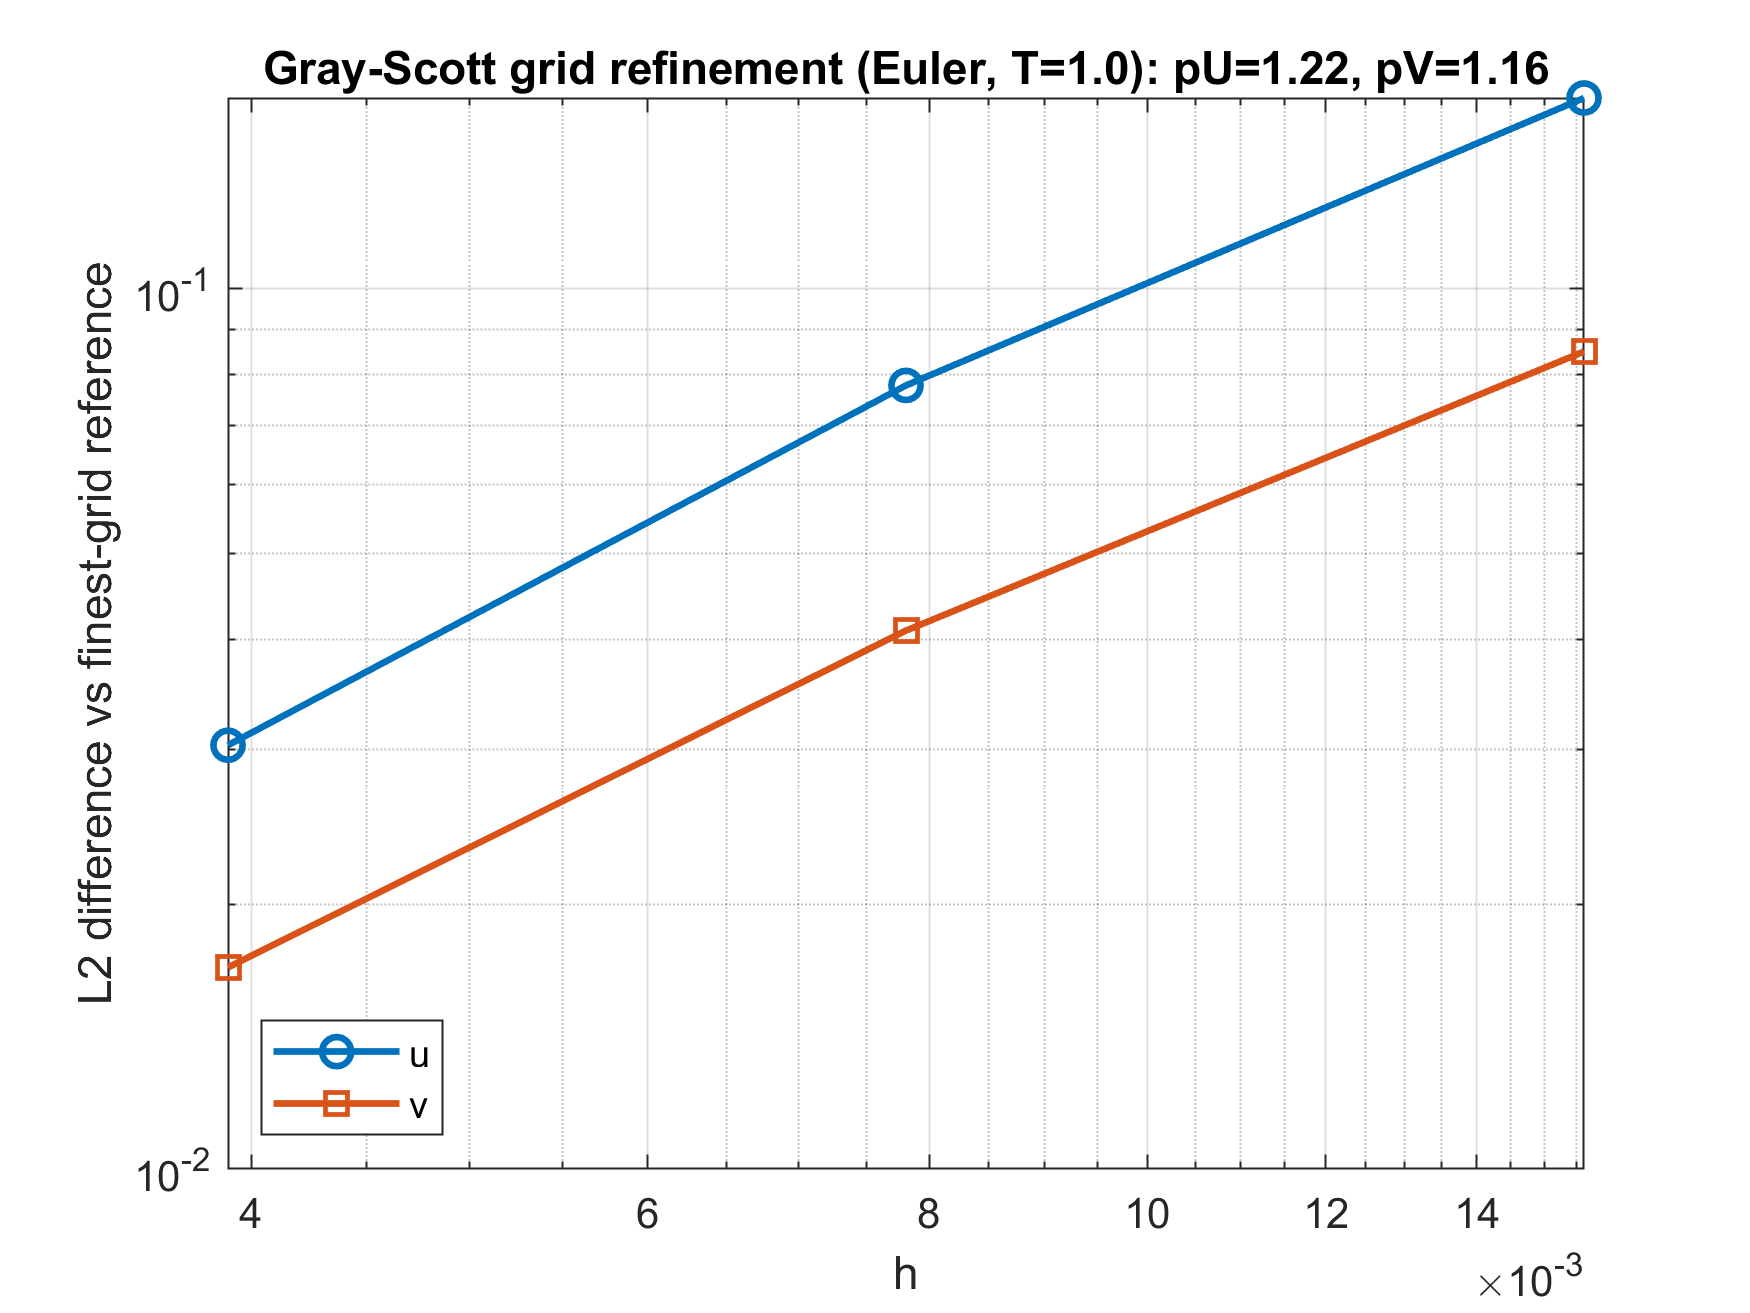
\includegraphics[width=0.82\textwidth]{figures/verification/grayscott_grid_refinement.png}
\caption{Final Gray--Scott grid-refinement study using the \(2048\times 2048\) solution as a numerical reference and a smooth grid-independent initial condition. The measured \(L^2\) differences in \(U\) and \(V\) decrease monotonically and yield observed rates \(p_U=p_V\approx 2.09\), consistent with second-order spatial behavior.}
\label{fig:grayscott_grid_refinement}
\end{figure}

\subsection{Test Case 8: Explicit Euler stability limit}
\label{sec:verification_testcase_explicit_stability_limit}

\paragraph{Aim.}
This test case verifies that the explicit Euler time integration used in the solver exhibits the correct conditional stability behavior for the diffusion part of the model. In contrast to the convergence tests, the purpose here is not to measure accuracy, but to check whether the implemented scheme obeys the theoretically known critical time-step limit. This is an important verification step because, for explicit methods, stability is a fundamental numerical property that must be reproduced correctly by the implementation.

\paragraph{Setup.}
The test is carried out in a controlled pure-diffusion subcase of the implemented Gray--Scott solver. To remove the reaction terms, the parameters are set to
\[
F = 0, \qquad k = 0,
\]
and the second species is initialized as
\[
v \equiv 0.
\]
As a result, the reaction part vanishes identically and the test isolates the explicit Euler discretization of the diffusion operator.

The computation is performed on a periodic square grid with
\[
N_x = N_y = 128.
\]
The diffusion coefficient of the first species is
\[
D_u = 2 \times 10^{-5},
\]
while \(D_v\) is irrelevant in this test because \(v\) remains zero throughout.

To excite the most restrictive mode for stability, the initial condition for \(u\) is chosen as a checkerboard perturbation around the constant mean state:
\[
u(x,y,0) = 1 + 0.1\,(-1)^{i+j}.
\]
This corresponds to the highest-frequency periodic mode of the discrete five-point Laplacian on an even grid. For this mode, the explicit Euler amplification factor is known analytically as
\[
g = 1 - \Delta t\,D_u\,\lambda_{\max},
\]
where
\[
\lambda_{\max} = \frac{4}{h_x^2} + \frac{4}{h_y^2}.
\]
Therefore, the critical time step is
\[
\Delta t_{\mathrm{crit}} = \frac{2}{D_u\,\lambda_{\max}}.
\]

For the documented run, this gives
\[
\Delta t_{\mathrm{crit}} = 0.762939.
\]
Three cases are then tested:
\[
\Delta t = 0.9\,\Delta t_{\mathrm{crit}}, \qquad
\Delta t = 1.0\,\Delta t_{\mathrm{crit}}, \qquad
\Delta t = 1.1\,\Delta t_{\mathrm{crit}}.
\]
Thus, the actual time-step values used are
\[
\Delta t \in \{0.68664551,\;0.76293945,\;0.83923340\}.
\]

Each case is advanced for
\[
n_{\text{steps}} = 20
\]
explicit Euler steps. At every step, the discrete \(L^2\) norm of the perturbation
\[
u - 1
\]
is measured. In addition to the observed one-step amplification factor, the complete measured norm history is compared against the theoretical history
\[
\|e^n\| = \|e^0\|\,|g|^n.
\]

\paragraph{How to run the test case.}
From the project \texttt{tests} folder, run:
\begin{verbatim}
r = test_explicit_stability_limit();
\end{verbatim}

The test prints the measured amplification factors and final norm ratios, and saves the generated figure in the local output folder of
\begin{verbatim}
tests/test_case_08_explicit_stability_limit/
\end{verbatim}

\paragraph{Expected result.}
For explicit Euler applied to diffusion, the expected behavior is classical:

\begin{itemize}
    \item if \(\Delta t < \Delta t_{\mathrm{crit}}\), the perturbation should decay;
    \item if \(\Delta t = \Delta t_{\mathrm{crit}}\), the perturbation norm should be preserved;
    \item if \(\Delta t > \Delta t_{\mathrm{crit}}\), the perturbation should grow, indicating instability.
\end{itemize}

For the chosen checkerboard mode, the theoretical one-step amplification factors are
\[
|g| = 0.8,\qquad 1.0,\qquad 1.2
\]
for the three tested cases. Therefore, the measured one-step amplification factors should agree with these values, and the full perturbation-norm history should follow the corresponding theoretical geometric behavior.

\paragraph{Obtained result.}
The test completed successfully, and the returned result was
\[
\texttt{pass} = 1.
\]

The MATLAB output reported:
\begin{verbatim}
case 1: dt = 0.68664551 = 0.90 dtCrit, g_theory = 0.800000,
        g_obs = 0.800000, final/initial = 0.011529,
        histRelErr = 3.247e-14

case 2: dt = 0.76293945 = 1.00 dtCrit, g_theory = 1.000000,
        g_obs = 1.000000, final/initial = 1.000000,
        histRelErr = 4.996e-15

case 3: dt = 0.83923340 = 1.10 dtCrit, g_theory = 1.200000,
        g_obs = 1.200000, final/initial = 38.337600,
        histRelErr = 9.415e-13
\end{verbatim}

The results are summarized in Table~\ref{tab:explicit_stability_limit}. In the subcritical case,
\[
\Delta t = 0.9\,\Delta t_{\mathrm{crit}},
\]
the perturbation decayed strongly, with final-to-initial ratio
\[
0.011529.
\]
At the critical value,
\[
\Delta t = \Delta t_{\mathrm{crit}},
\]
the perturbation norm was preserved exactly:
\[
\frac{\|e^{20}\|}{\|e^0\|} = 1.
\]
In the supercritical case,
\[
\Delta t = 1.1\,\Delta t_{\mathrm{crit}},
\]
the perturbation grew rapidly, with final-to-initial ratio
\[
38.337600.
\]

Most importantly, the measured one-step amplification factors matched the theoretical values exactly in all three cases:
\[
g_{\mathrm{obs}} = g_{\mathrm{theory}} = \{0.8,\;1.0,\;1.2\}.
\]
Moreover, the maximum relative error between the complete measured norm history and the theoretical geometric history remained extremely small, with worst case
\[
9.415 \times 10^{-13}.
\]

\begin{table}[htbp]
\centering
\caption{Explicit Euler stability-limit test results for the diffusion subcase on the \(128\times128\) periodic grid.}
\label{tab:explicit_stability_limit}
\begin{tabular}{|c|c|c|c|c|}
\hline
Case & \(\Delta t / \Delta t_{\mathrm{crit}}\) & \(g_{\mathrm{theory}}\) & \(g_{\mathrm{obs}}\) & final/initial \\
\hline
stable     & 0.9 & 0.8 & 0.8 & 0.011529 \\
critical   & 1.0 & 1.0 & 1.0 & 1.000000 \\
unstable   & 1.1 & 1.2 & 1.2 & 38.337600 \\
\hline
\end{tabular}
\end{table}

Figure~\ref{fig:explicit_stability_limit} shows the normalized perturbation \(L^2\) norm as a function of Euler step. The subcritical case decays monotonically, the critical case remains constant, and the supercritical case grows exponentially. The figure therefore reproduces exactly the three theoretical stability regimes expected for the explicit Euler discretization of diffusion.

Hence, this test confirms that the implementation reproduces the correct stability boundary of the explicit Euler method. It verifies not only the qualitative behavior below, at, and above the critical time step, but also the quantitative amplification factors predicted by theory.

\begin{figure}[htbp]
\centering
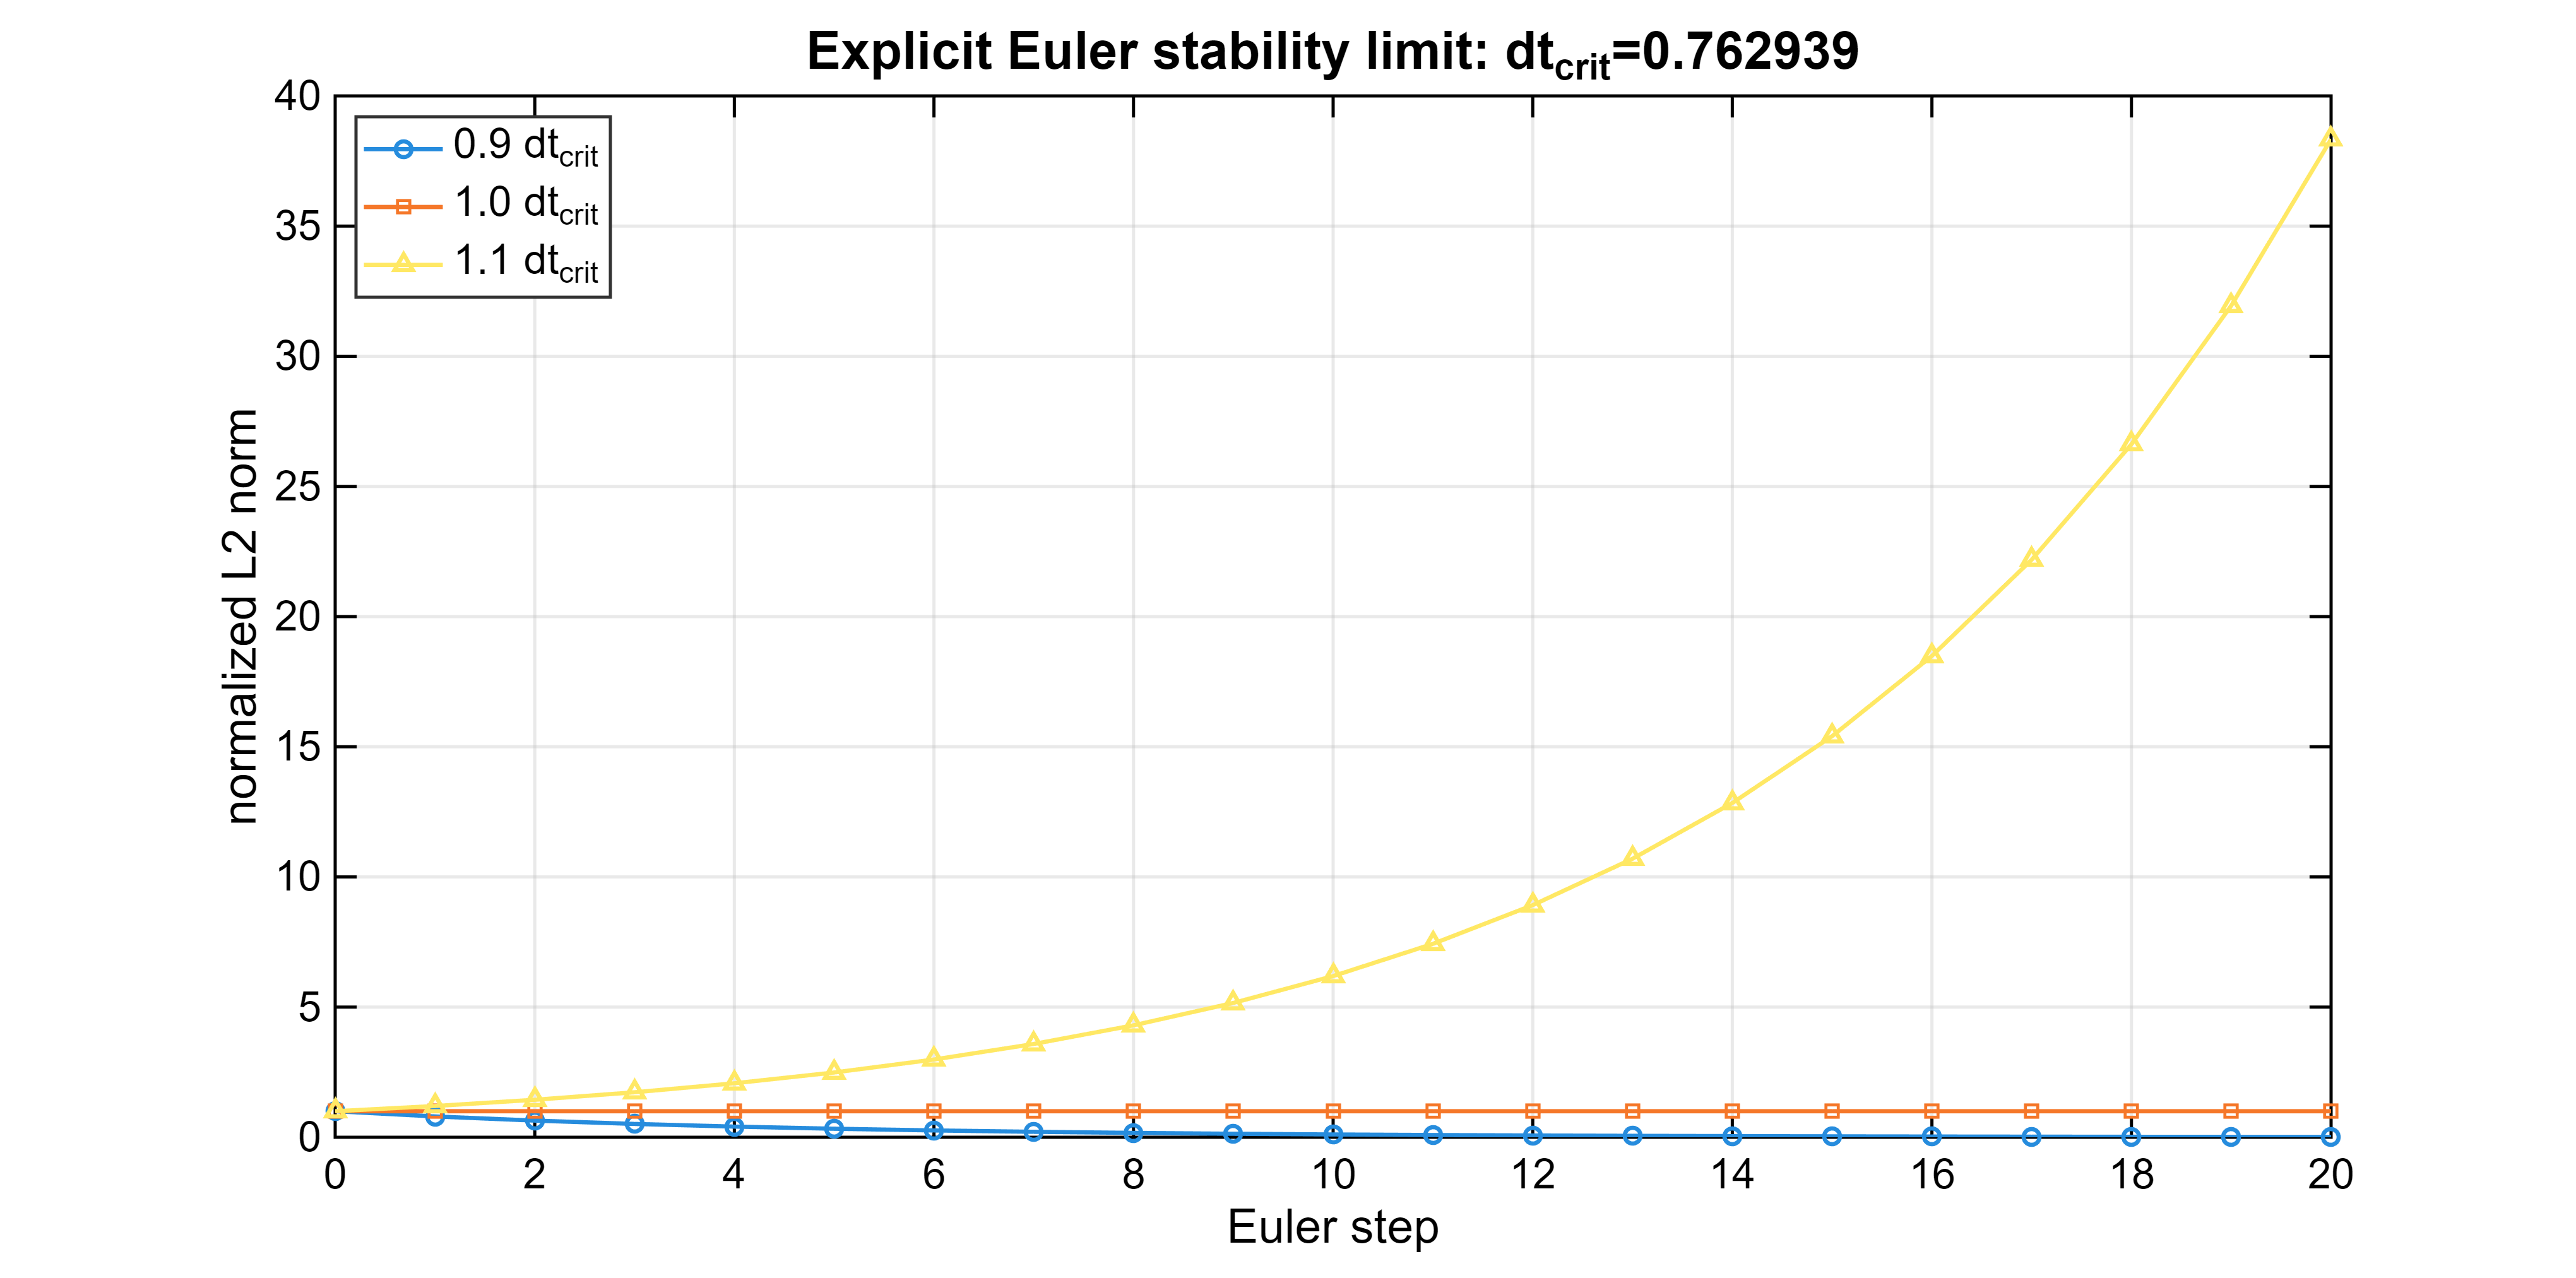
\includegraphics[width=0.82\textwidth]{figures/verification/explicit_stability_limit.png}
\caption{Explicit Euler stability-limit test for the diffusion subcase on the \(128\times128\) periodic grid. Below the critical time step the perturbation decays, at the critical value it is preserved, and above the critical value it grows, in exact agreement with the theoretical amplification factors.}
\label{fig:explicit_stability_limit}
\end{figure}

\section{Supplementary verification checks}
\label{sec:verification_supplementary}

In addition to the detailed test cases above, several smaller checks were carried out to support the overall verification strategy. These tests are useful because they isolate specific mathematical or implementation properties, even if they do not require a full standalone discussion.

\subsection{Constant-field Laplacian null test}
\label{sec:verification_constant_field}

As an additional structural check, the discrete Laplacian was applied to a constant field. For a constant function, the continuous Laplacian is identically zero, and the same property is expected from the discrete operator. Therefore, this test serves as a simple but useful sanity check of the assembled diffusion operator.

The test was executed with:
\begin{verbatim}
r = test_laplacian_constant();
\end{verbatim}

For the documented run, the returned result was
\[
\texttt{pass} = 1,
\]
with
\[
\|L\mathbf{1}\|_{\infty} = 0.000\times 10^{0},
\qquad
\|L\mathbf{1}\|_{2} = 0.000\times 10^{0}.
\]
Thus, the discrete Laplacian annihilates a constant field exactly in this case. This confirms that the operator satisfies an important basic consistency property and provides additional evidence that the diffusion discretization is assembled correctly.

\subsection{Symmetry check of the discrete Laplacian matrix}
\label{sec:verification_laplacian_symmetry}

A further structural verification step checks the symmetry of the assembled discrete Laplacian matrix. For the periodic finite-difference diffusion operator used in this project, the Laplacian matrix is expected to be symmetric under the tested setup. This property is important because it supports the correctness of the stencil-to-matrix assembly and helps detect indexing or coefficient-placement errors.

The test was executed with:
\begin{verbatim}
r = test_laplacian_symmetry();
\end{verbatim}

For the documented run, the returned result was
\[
\texttt{pass} = 1,
\]
and the reported symmetry defect was
\[
\|L - L^{T}\|_{\infty} = 0.000\times 10^{0}.
\]
Therefore, the assembled Laplacian matrix is exactly symmetric in this case. This result is fully consistent with the expected structure of the periodic diffusion operator and provides additional evidence that the matrix assembly is implemented correctly.

\subsection{End-to-end MMS consistency check}
\label{sec:verification_mms_endtoend}

As a supplementary verification step, the full solver was tested with a manufactured-solution setup. In contrast to the operator-only MMS test of Test Case~1, this check verifies the complete time-dependent workflow, including reaction, diffusion, source-term handling, and explicit Euler time stepping. It is therefore useful as supporting end-to-end verification evidence for the implemented numerical model.

The test was executed with:
\begin{verbatim}
r = test_mms_endtoend();
\end{verbatim}

For the documented run, the solver used a grid
\[
N_x=N_y=128,
\]
a time step
\[
\Delta t = 0.01,
\]
and a final time
\[
T = 1.
\]
The returned result was
\[
\texttt{pass} = 1,
\]
and the reported final \(L^2\) errors were
\[
\mathrm{err}_U^{L^2} = 1.179\times 10^{-4},
\qquad
\mathrm{err}_V^{L^2} = 5.974\times 10^{-4}.
\]

These errors are small for the chosen grid and time-step size. They are consistent with a correctly implemented manufactured-solution workflow. The generated error figure is stored in the local output folder of \texttt{tests/supplementary\_checks/}. Figure~\ref{fig:mms_endtoend_errV} shows the spatial error field for \(v\) at the final time. The smooth, structured pattern is typical of discretization error and does not indicate instability or implementation failure.

\begin{figure}[htbp]
\centering
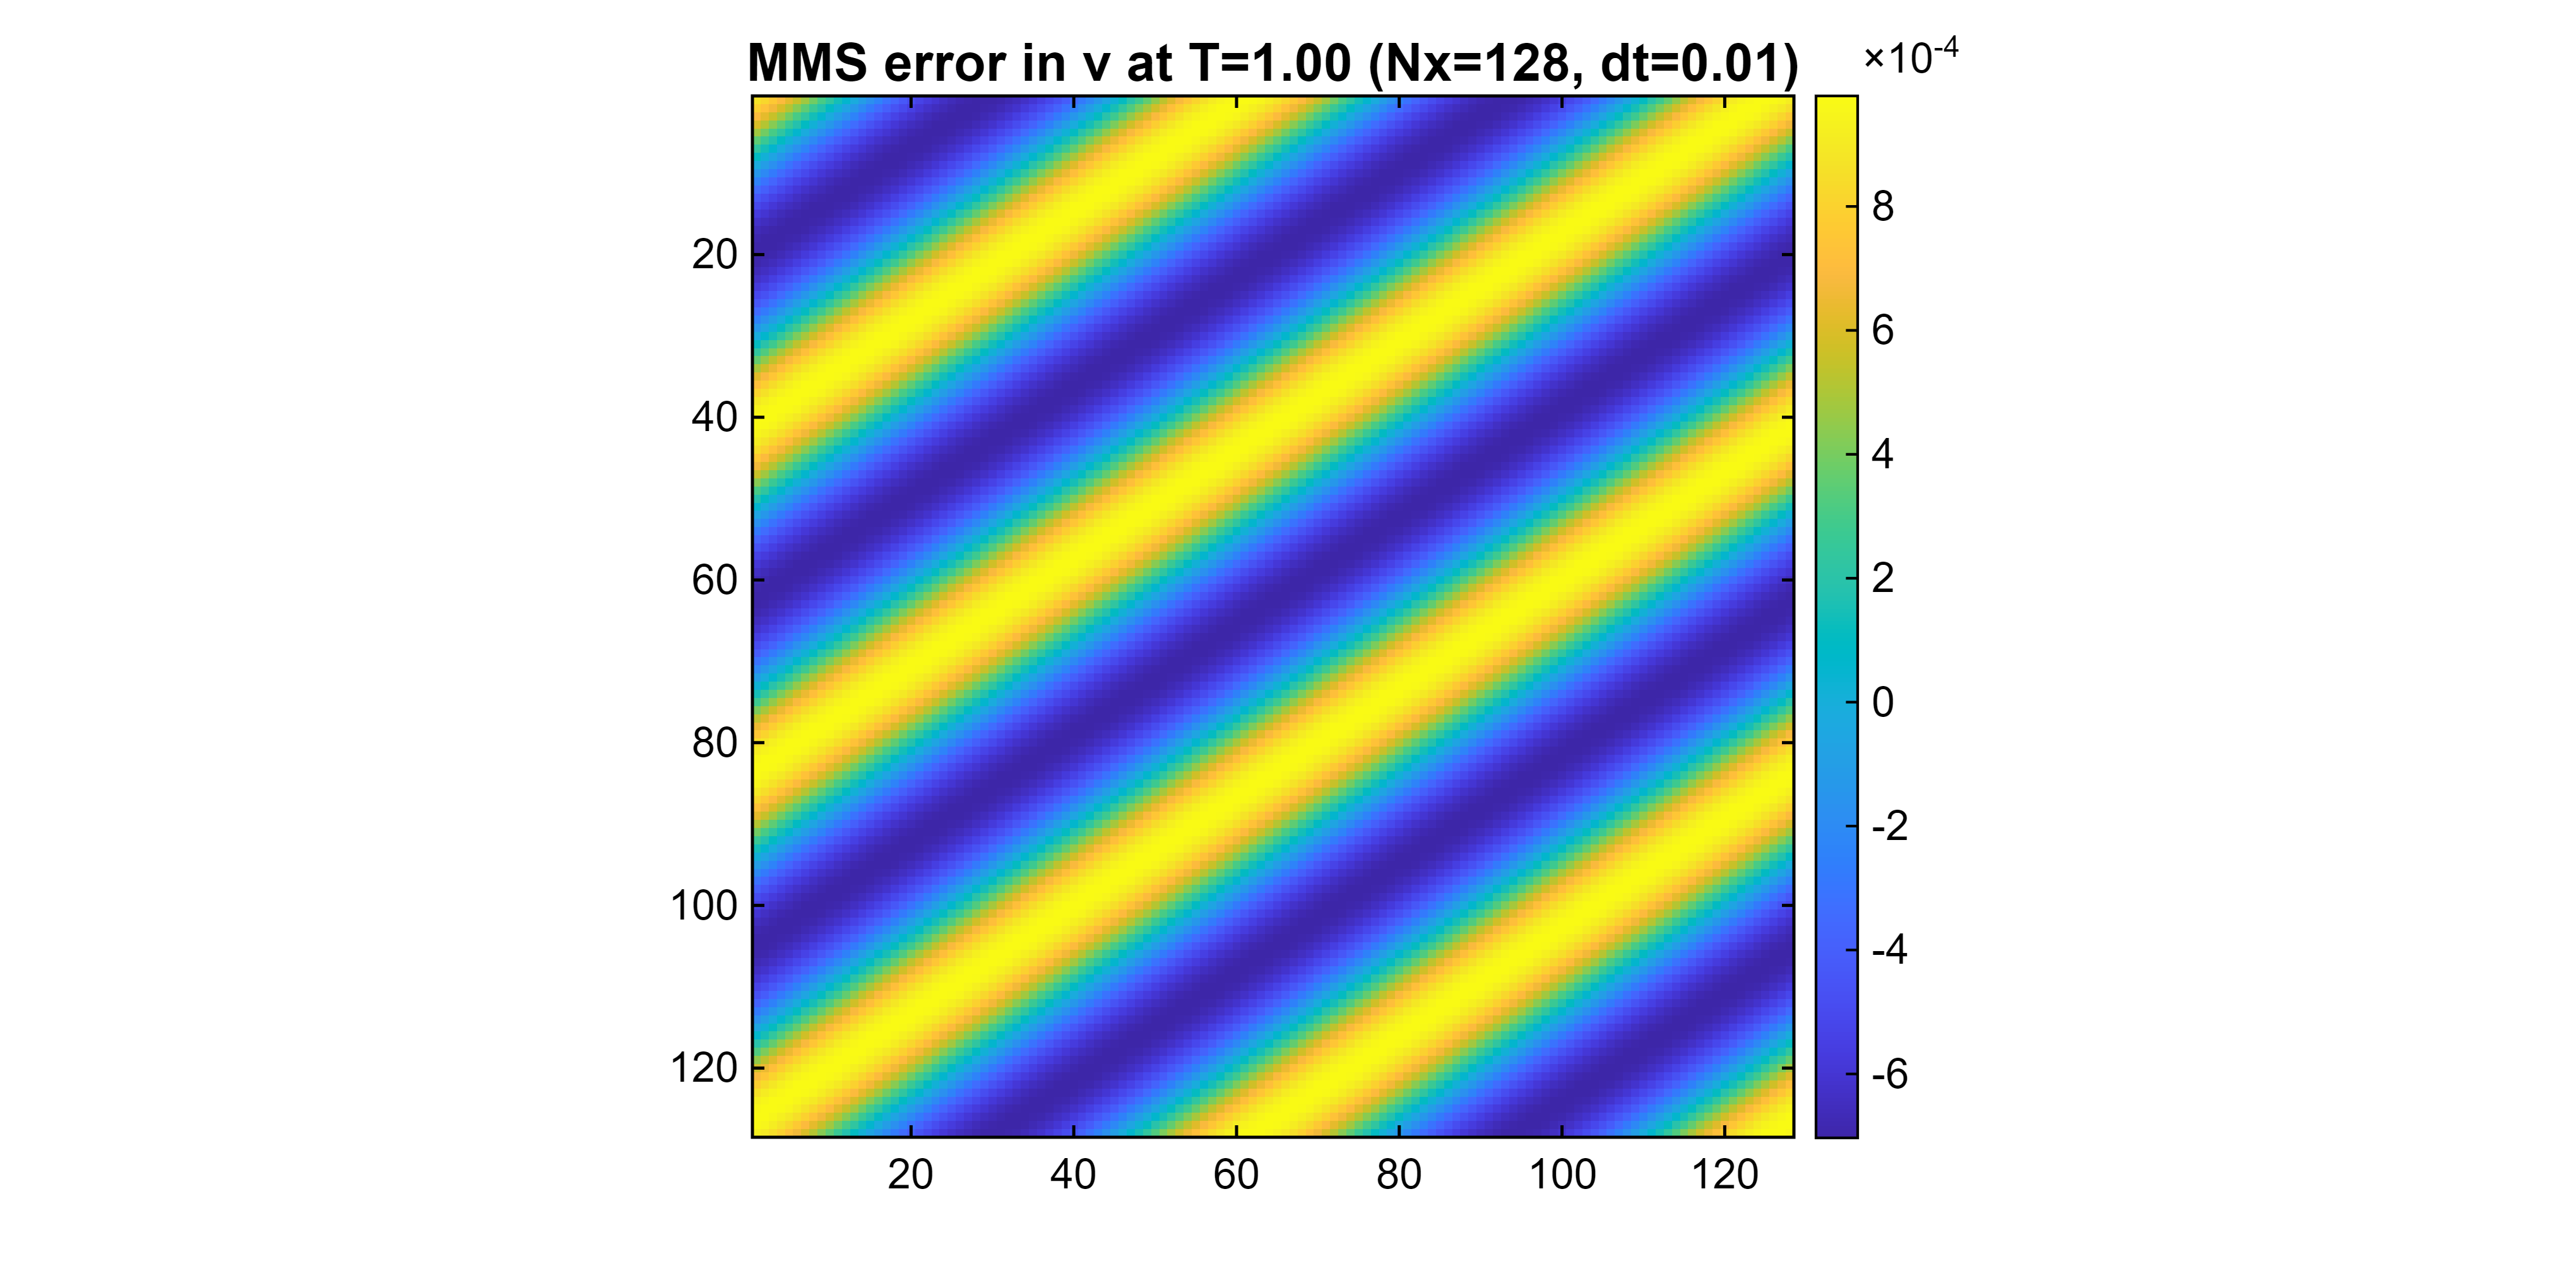
\includegraphics[width=0.72\textwidth]{figures/verification/mms_endtoend_errV.png}
\caption{Spatial error field of the manufactured-solution end-to-end test for \(v\) at \(T=1\), with \(N_x=N_y=128\) and \(\Delta t=0.01\).}
\label{fig:mms_endtoend_errV}
\end{figure}

Overall, this supplementary test provides additional evidence that the complete solver reproduces the manufactured solution with small final errors when the corresponding source terms are included.

\subsection{Time-step halving smoke test}
\label{sec:verification_timestep_halving_smoke}

As a quick supplementary consistency check, a simpler time-step halving test was also performed. In contrast to the full temporal convergence study of Test Case~2, this test is not intended as a rigorous order-verification procedure. Instead, it serves as a compact sanity check showing that the numerical solution changes in the expected direction when the time step is refined.

The test was executed with:
\begin{verbatim}
r = test_timestep_halving_smoke();
\end{verbatim}

For the documented run, the solver used a grid
\[
N_x=N_y=128,
\]
a final time
\[
T=50,
\]
and the baseline time step
\[
\Delta t = 0.2.
\]
The returned result was
\[
\texttt{pass} = 1,
\]
and the reported differences between successive refinements were
\[
\mathrm{rms}_{12} = 3.706\times 10^{-5}, \qquad
\mathrm{rms}_{24} = 1.851\times 10^{-5},
\]
\[
\mathrm{inf}_{12} = 5.798\times 10^{-4}, \qquad
\mathrm{inf}_{24} = 2.891\times 10^{-4}.
\]

The finer-step differences are smaller than the coarser-step differences in both norms:
\[
\mathrm{rms}_{24} < \mathrm{rms}_{12},
\qquad
\mathrm{inf}_{24} < \mathrm{inf}_{12}.
\]
Moreover, the reduction is approximately by a factor of two, which is consistent with the expected first-order behavior of the explicit Euler method under time-step halving.


\section{Validation-oriented pattern sanity check}
\label{sec:verification_pattern_sanity}

In addition to the formal verification tests presented earlier in this chapter, a long-time Gray--Scott pattern study was carried out as a \emph{validation-oriented sanity check}. The role of this section is intentionally different from that of the preceding test cases. The earlier tests were designed to verify numerical correctness in a strict sense, for example through manufactured solutions, convergence measurements, operator equivalence, boundary-condition enforcement, and consistency checks between different execution paths. By contrast, the present study asks whether the implemented solver also reproduces the kind of plausible and morphologically distinct pattern classes that are commonly associated with the Gray--Scott model in the literature.

The Gray--Scott system is well known for producing a rich variety of self-organized structures depending on the feed and kill parameters. Pearson's classical study established the basic pattern-forming context of the model, while later classification work organized a broader range of visually distinct regimes using labels such as \texttt{alpha}, \texttt{epsilon}, \texttt{kappa}, and \texttt{theta} \cite{pearson1993,munafo_gray_scott_classes}. A modern tutorial-style analysis of the Gray--Scott model and its pattern behavior is also given in \cite{gandy2022}. The present test is therefore not intended to replace the formal verification evidence, but rather to complement it by showing that the final implementation produces stable and qualitatively reasonable long-time dynamics for standard Pearson-type parameter choices.

\subsection{Test Case 9: Pearson-type pattern sanity check}
\label{sec:verification_testcase_pearson}

\paragraph{Aim.}
This test case checks whether the implemented solver reproduces visually reasonable Gray--Scott patterns for several Pearson-type parameter sets over a long simulation horizon. The aim is not to verify a convergence order or to compare against an exact analytical solution, but to confirm that the final implementation is capable of producing the expected diversity of Gray--Scott morphologies under standard long-time conditions. More specifically, the test examines whether different parameter choices lead to clearly different and stable pattern classes rather than to numerical noise, spurious artifacts, or an incorrect collapse to a trivial state.

\paragraph{Setup.}
The test uses the Pearson preset on the periodic square domain
\[
\Omega = [0,1)\times[0,1)
\]
with a uniform grid
\[
N_x = N_y = 256.
\]
The time step is
\[
\Delta t = 1,
\]
and each case is simulated for
\[
N_t = 200000
\]
time steps, corresponding to the final time
\[
T = 200000.
\]
The diffusion coefficients are
\[
D_u = 2\times 10^{-5}, \qquad D_v = 1\times 10^{-5},
\]
and periodic boundary conditions are imposed on all sides.

Four Pearson-type parameter sets are tested:
\[
\texttt{alpha}: \quad F=0.0075294,\qquad k=0.04564,
\]
\[
\texttt{kappa}: \quad F=0.034487,\qquad k=0.060378,
\]
\[
\texttt{epsilon}: \quad F=0.019707,\qquad k=0.055379,
\]
\[
\texttt{theta}: \quad F=0.040117,\qquad k=0.060515.
\]

For each case, snapshots of the \(U\)- and \(V\)-fields are saved at
\[
t = 50000,\;100000,\;150000,\;200000.
\]
In the present report, the \(U\)-field snapshots at
\[
t = 100000
\]
are used for comparison, because at this time the morphology of each case is already well developed while still being easy to interpret visually.

\paragraph{How to run the test case.}
From the project \texttt{tests} folder, run:
\begin{verbatim}
r = test_pattern_sanity_pearson();
\end{verbatim}

The test saves the generated images in the local output folder of
\begin{verbatim}
tests/test_case_09_pearson_pattern_sanity/
\end{verbatim}
and, for the documented run, completed all four cases successfully. The MATLAB output reported that snapshots were saved for all four parameter sets at
\[
t=50000,\;100000,\;150000,\;200000,
\]
and that the full run finished for the cases
\[
\texttt{alpha},\;\texttt{kappa},\;\texttt{epsilon},\;\texttt{theta}.
\]

\paragraph{Expected result.}
Since this is a validation-oriented sanity check, the expected result is qualitative rather than pointwise exact. One expects the simulation to produce stable, visually structured Gray--Scott patterns whose morphology depends strongly on the chosen \((F,k)\) pair. In particular, different Pearson-type labels should not all lead to nearly identical images. Instead, some cases should favor spot-dominated structures, while others should exhibit more elongated stripe-like or labyrinthine organizations \cite{pearson1993,munafo_gray_scott_classes}. The important criterion is therefore not exact agreement with a single published image, but rather the emergence of distinct and plausible pattern classes under long-time integration. As a supporting modern reference, \cite{gandy2022} also discusses the sensitivity of Gray--Scott pattern formation to parameter choice.

\paragraph{Obtained result.}
The test completed successfully, and the returned result was
\[
\texttt{pass} = 1.
\]
Each of the four parameter sets was simulated over the full
\[
200000
\]
time steps, and all requested snapshots were saved.
The representative \(U\)-field snapshots at \(t=100000\), shown in Figs.~\ref{fig:pearson_alpha_snapshot}--\ref{fig:pearson_theta_snapshot}, demonstrate that the implemented solver generates clearly different and visually plausible pattern morphologies for the four tested parameter sets.

The \texttt{alpha} case in Fig.~\ref{fig:pearson_alpha_snapshot} is dominated by separated spot-like structures embedded in a mostly high-\(U\) background. The spots are irregularly distributed, but they remain localized and well formed. The image does not suggest numerical breakup, grid-aligned artifacts, or unstable oscillatory contamination. Instead, it shows a coherent spot-dominated regime consistent with the expected Gray--Scott behavior for this type of parameter choice.

The \texttt{epsilon} case in Fig.~\ref{fig:pearson_epsilon_snapshot} also belongs to a spot-dominated family, but the pattern is markedly denser and more crowded than in the \texttt{alpha} case. Small spot-like depressions in the \(U\)-field are distributed much more uniformly across the domain, producing a texture that is finer and more tightly packed. This visual difference is important because it shows that the solver is not merely reproducing one generic spot pattern for all parameter values; rather, it responds sensitively to the change in \((F,k)\) and produces a distinctly different morphological regime.

By contrast, the \texttt{kappa} case in Fig.~\ref{fig:pearson_kappa_snapshot} is no longer spot-dominated. Instead, the solution organizes into broad, elongated, stripe-like structures with a labyrinthine appearance. The stripes are smooth and continuous over long distances, and they form an interconnected network rather than isolated islands. This is a qualitatively different regime from the previous two cases and is visually consistent with the classic Gray--Scott transition from spot patterns to stripe or maze-like patterns under different parameter settings.

The \texttt{theta} case in Fig.~\ref{fig:pearson_theta_snapshot} is also labyrinth-like, but it is not identical to \texttt{kappa}. The stripe network is more intricate and locally more curved, and the overall topology appears somewhat more tangled and fine-scaled. Thus, even within the stripe-dominated family, the implementation still distinguishes between parameter sets and produces visibly different structure. This strengthens the interpretation that the solver is capturing meaningful qualitative pattern dependence rather than generating a single repeated texture.

Taken together, these four cases show two important features. First, the runs remain numerically stable and visually clean over a very long integration horizon. Second, the parameter changes lead to clear morphological differentiation between spot-dominated and labyrinth-dominated regimes, with further variation inside each family. This is exactly the kind of application-level behavior expected from a plausible Gray--Scott implementation \cite{pearson1993,munafo_gray_scott_classes}.

At the same time, the interpretation of this test should remain careful. Because no exact reference field is available, the present result does not prove correctness in the same way as the manufactured-solution or convergence-based tests. Its role is supportive: it shows that the implemented model behaves plausibly, produces stable long-time structures, and reproduces the qualitative diversity associated with Pearson-type Gray--Scott dynamics.

\begin{figure}[htbp]
\centering
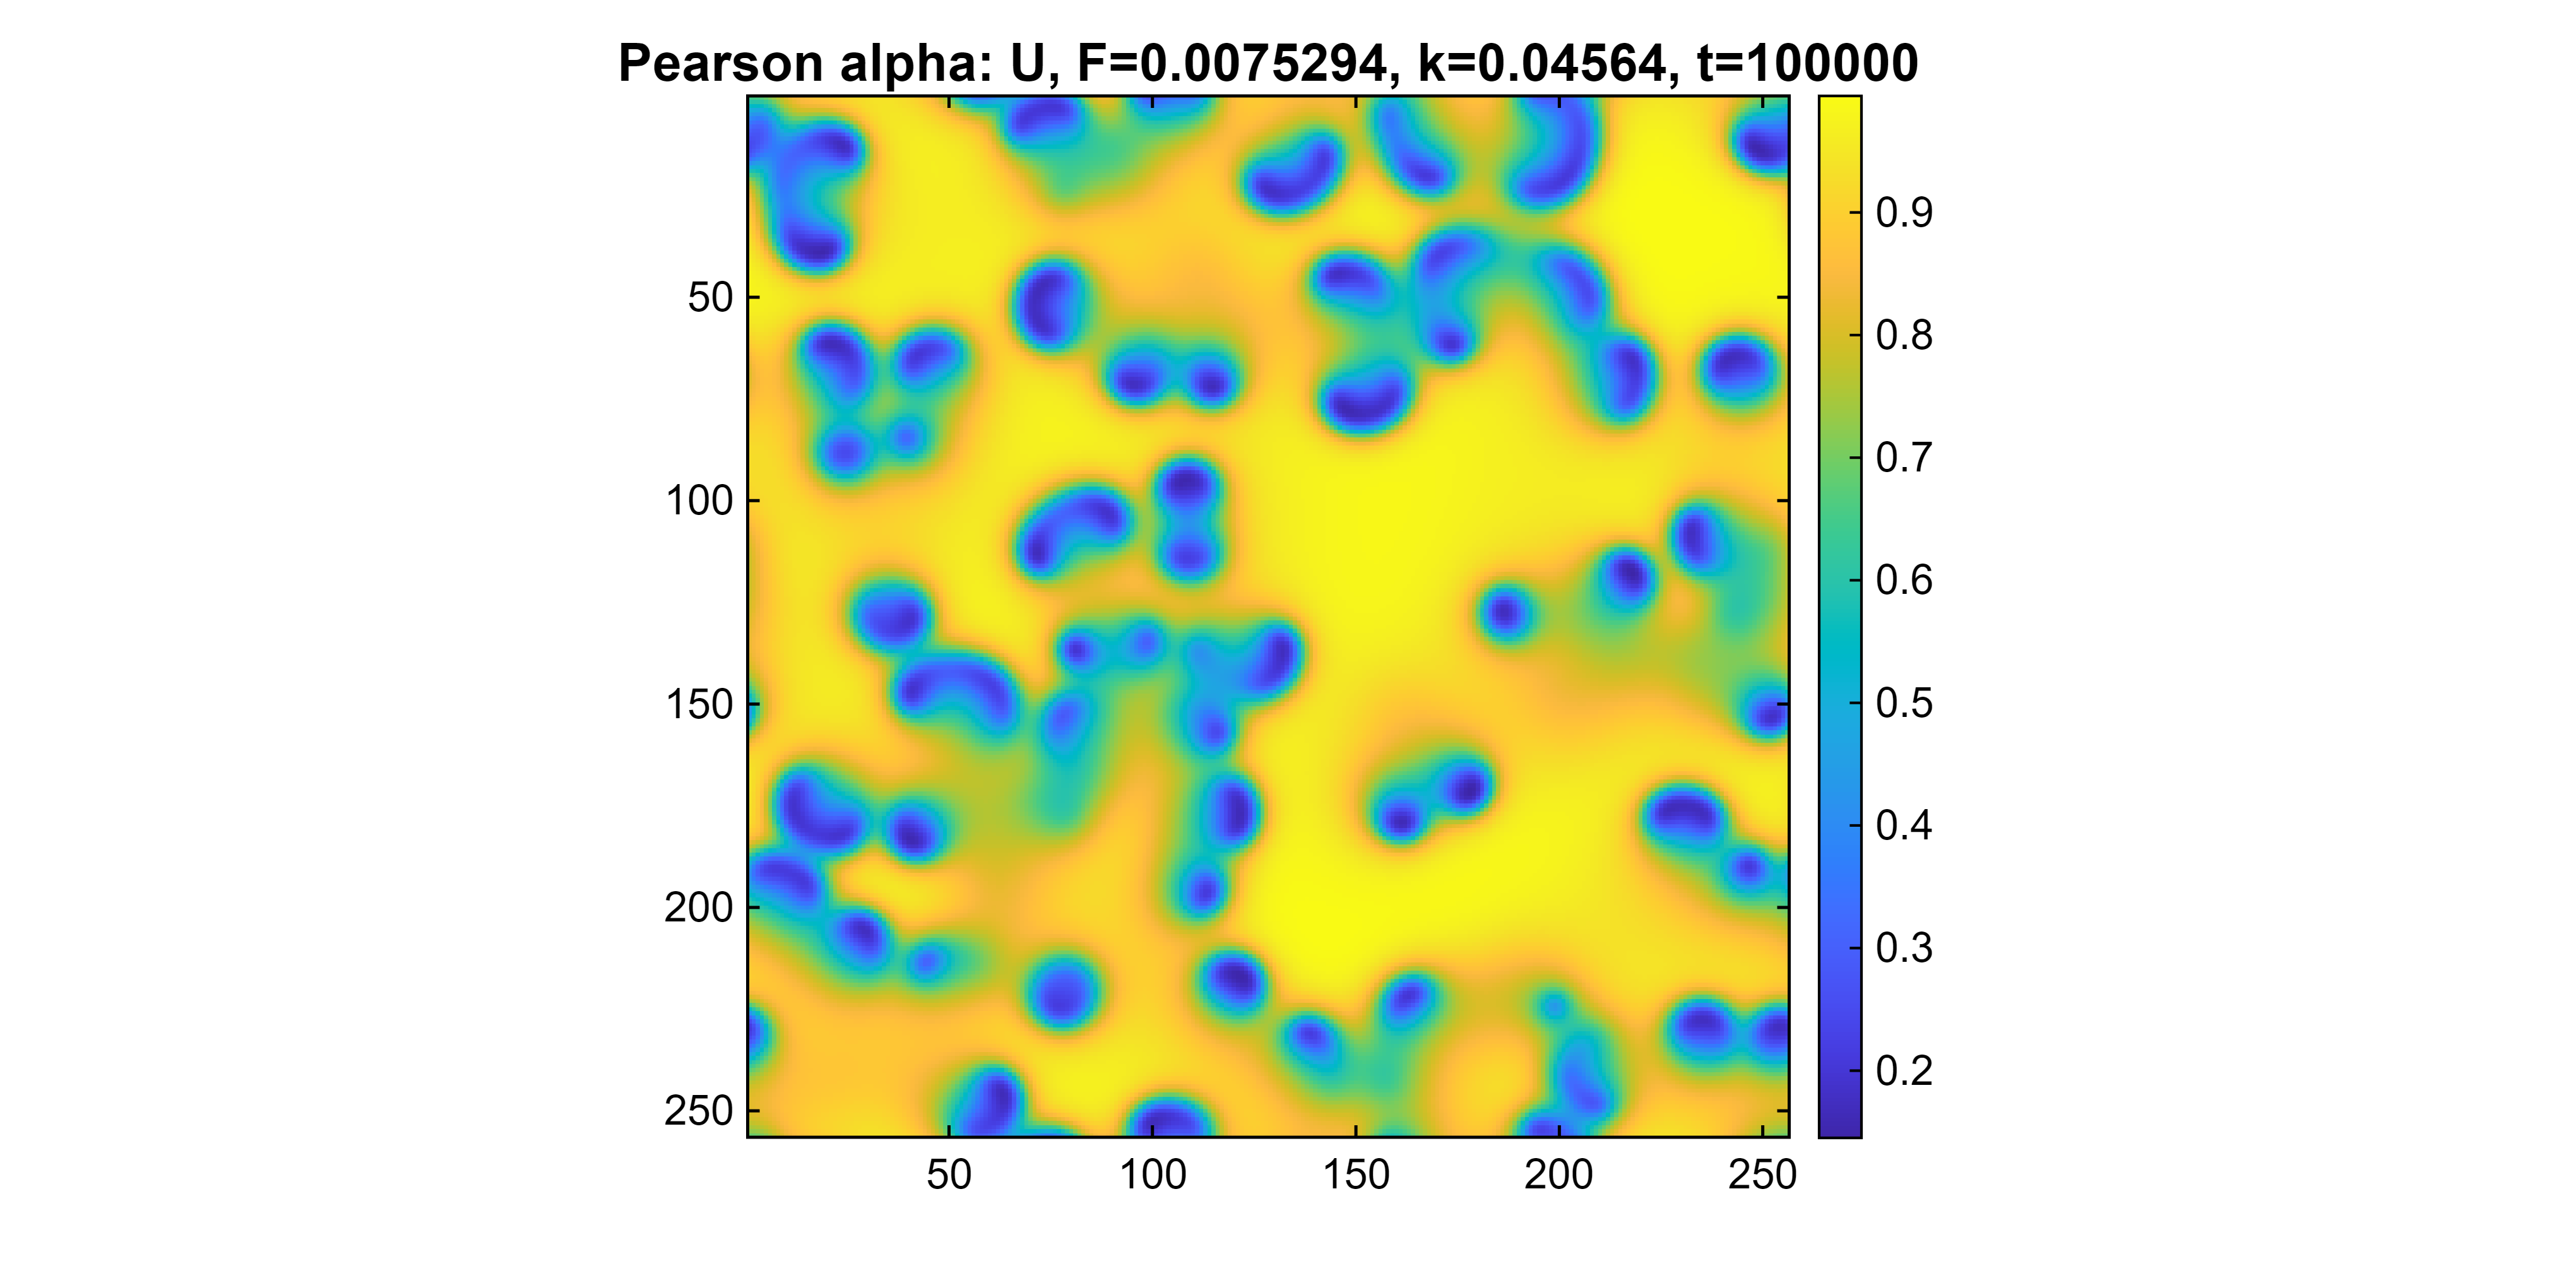
\includegraphics[width=0.95\textwidth]{figures/verification/pattern_sanity/alpha_t100000_U.png}
\caption{Pearson \texttt{alpha} case: representative \(U\)-field snapshot at \(t=100000\). The morphology is dominated by separated spot-like structures in a mostly high-\(U\) background.}
\label{fig:pearson_alpha_snapshot}
\end{figure}

\begin{figure}[htbp]
\centering
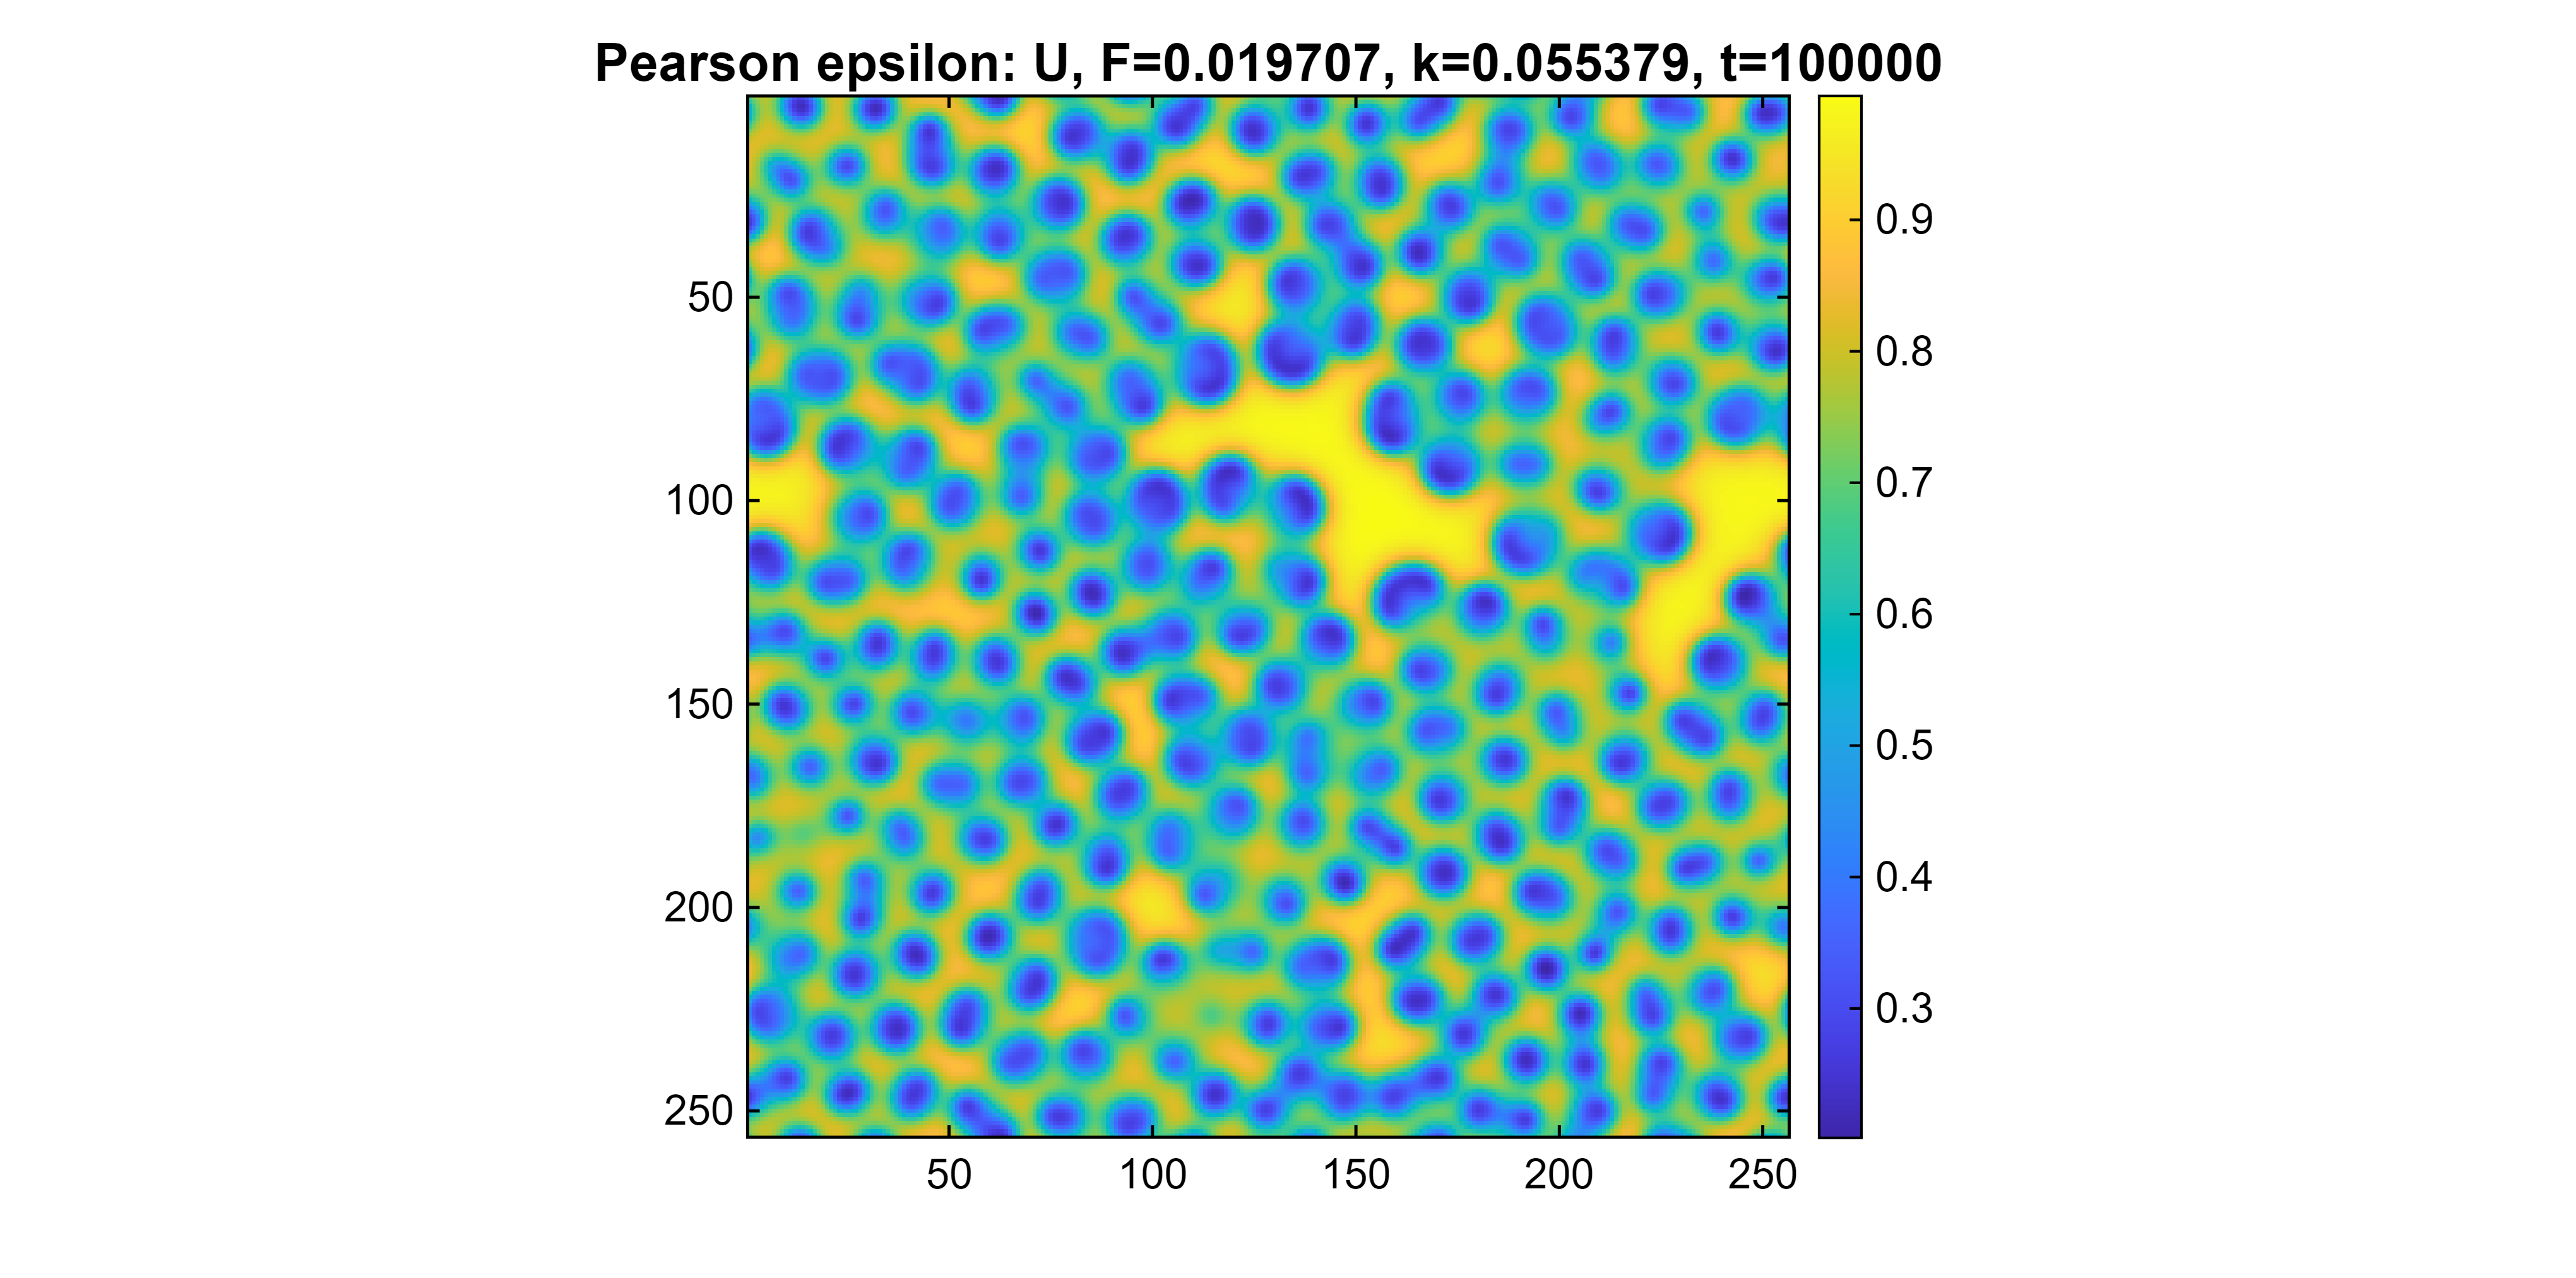
\includegraphics[width=0.95\textwidth]{figures/verification/pattern_sanity/epsilon_t100000_U.png}
\caption{Pearson \texttt{epsilon} case: representative \(U\)-field snapshot at \(t=100000\). Compared with \texttt{alpha}, the pattern is denser and more uniformly populated by small spot-like structures.}
\label{fig:pearson_epsilon_snapshot}
\end{figure}

\begin{figure}[htbp]
\centering
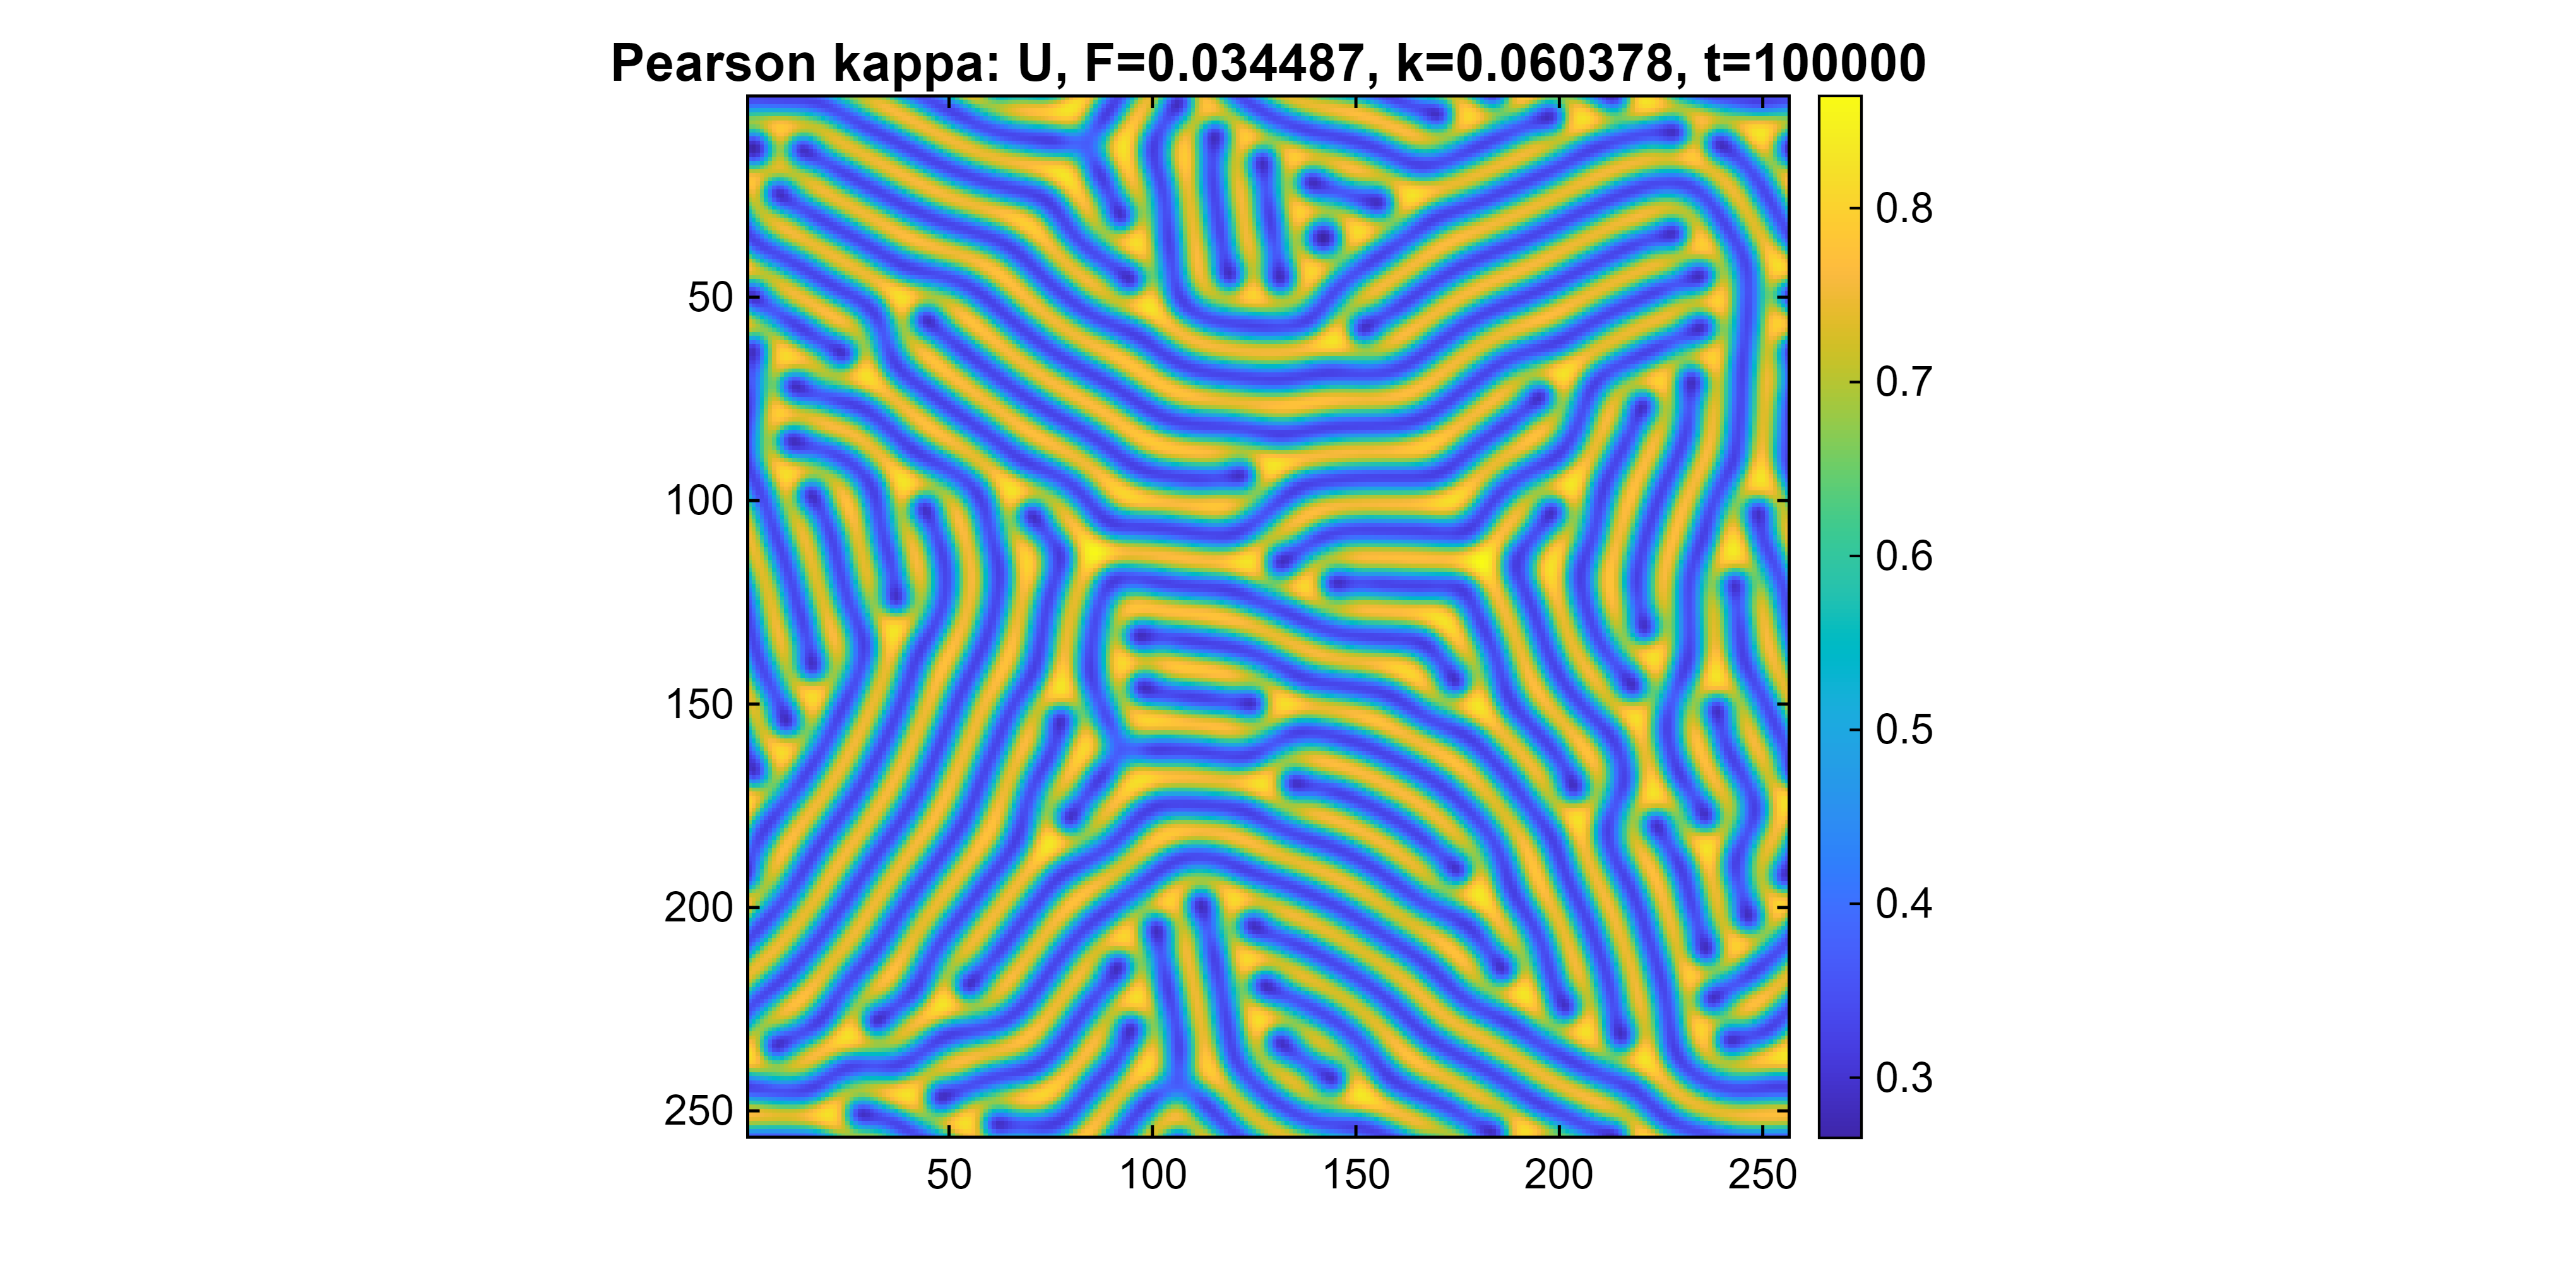
\includegraphics[width=0.95\textwidth]{figures/verification/pattern_sanity/kappa_t100000_U.png}
\caption{Pearson \texttt{kappa} case: representative \(U\)-field snapshot at \(t=100000\). The pattern exhibits a broad labyrinth-like stripe morphology rather than isolated spots.}
\label{fig:pearson_kappa_snapshot}
\end{figure}

\begin{figure}[htbp]
\centering
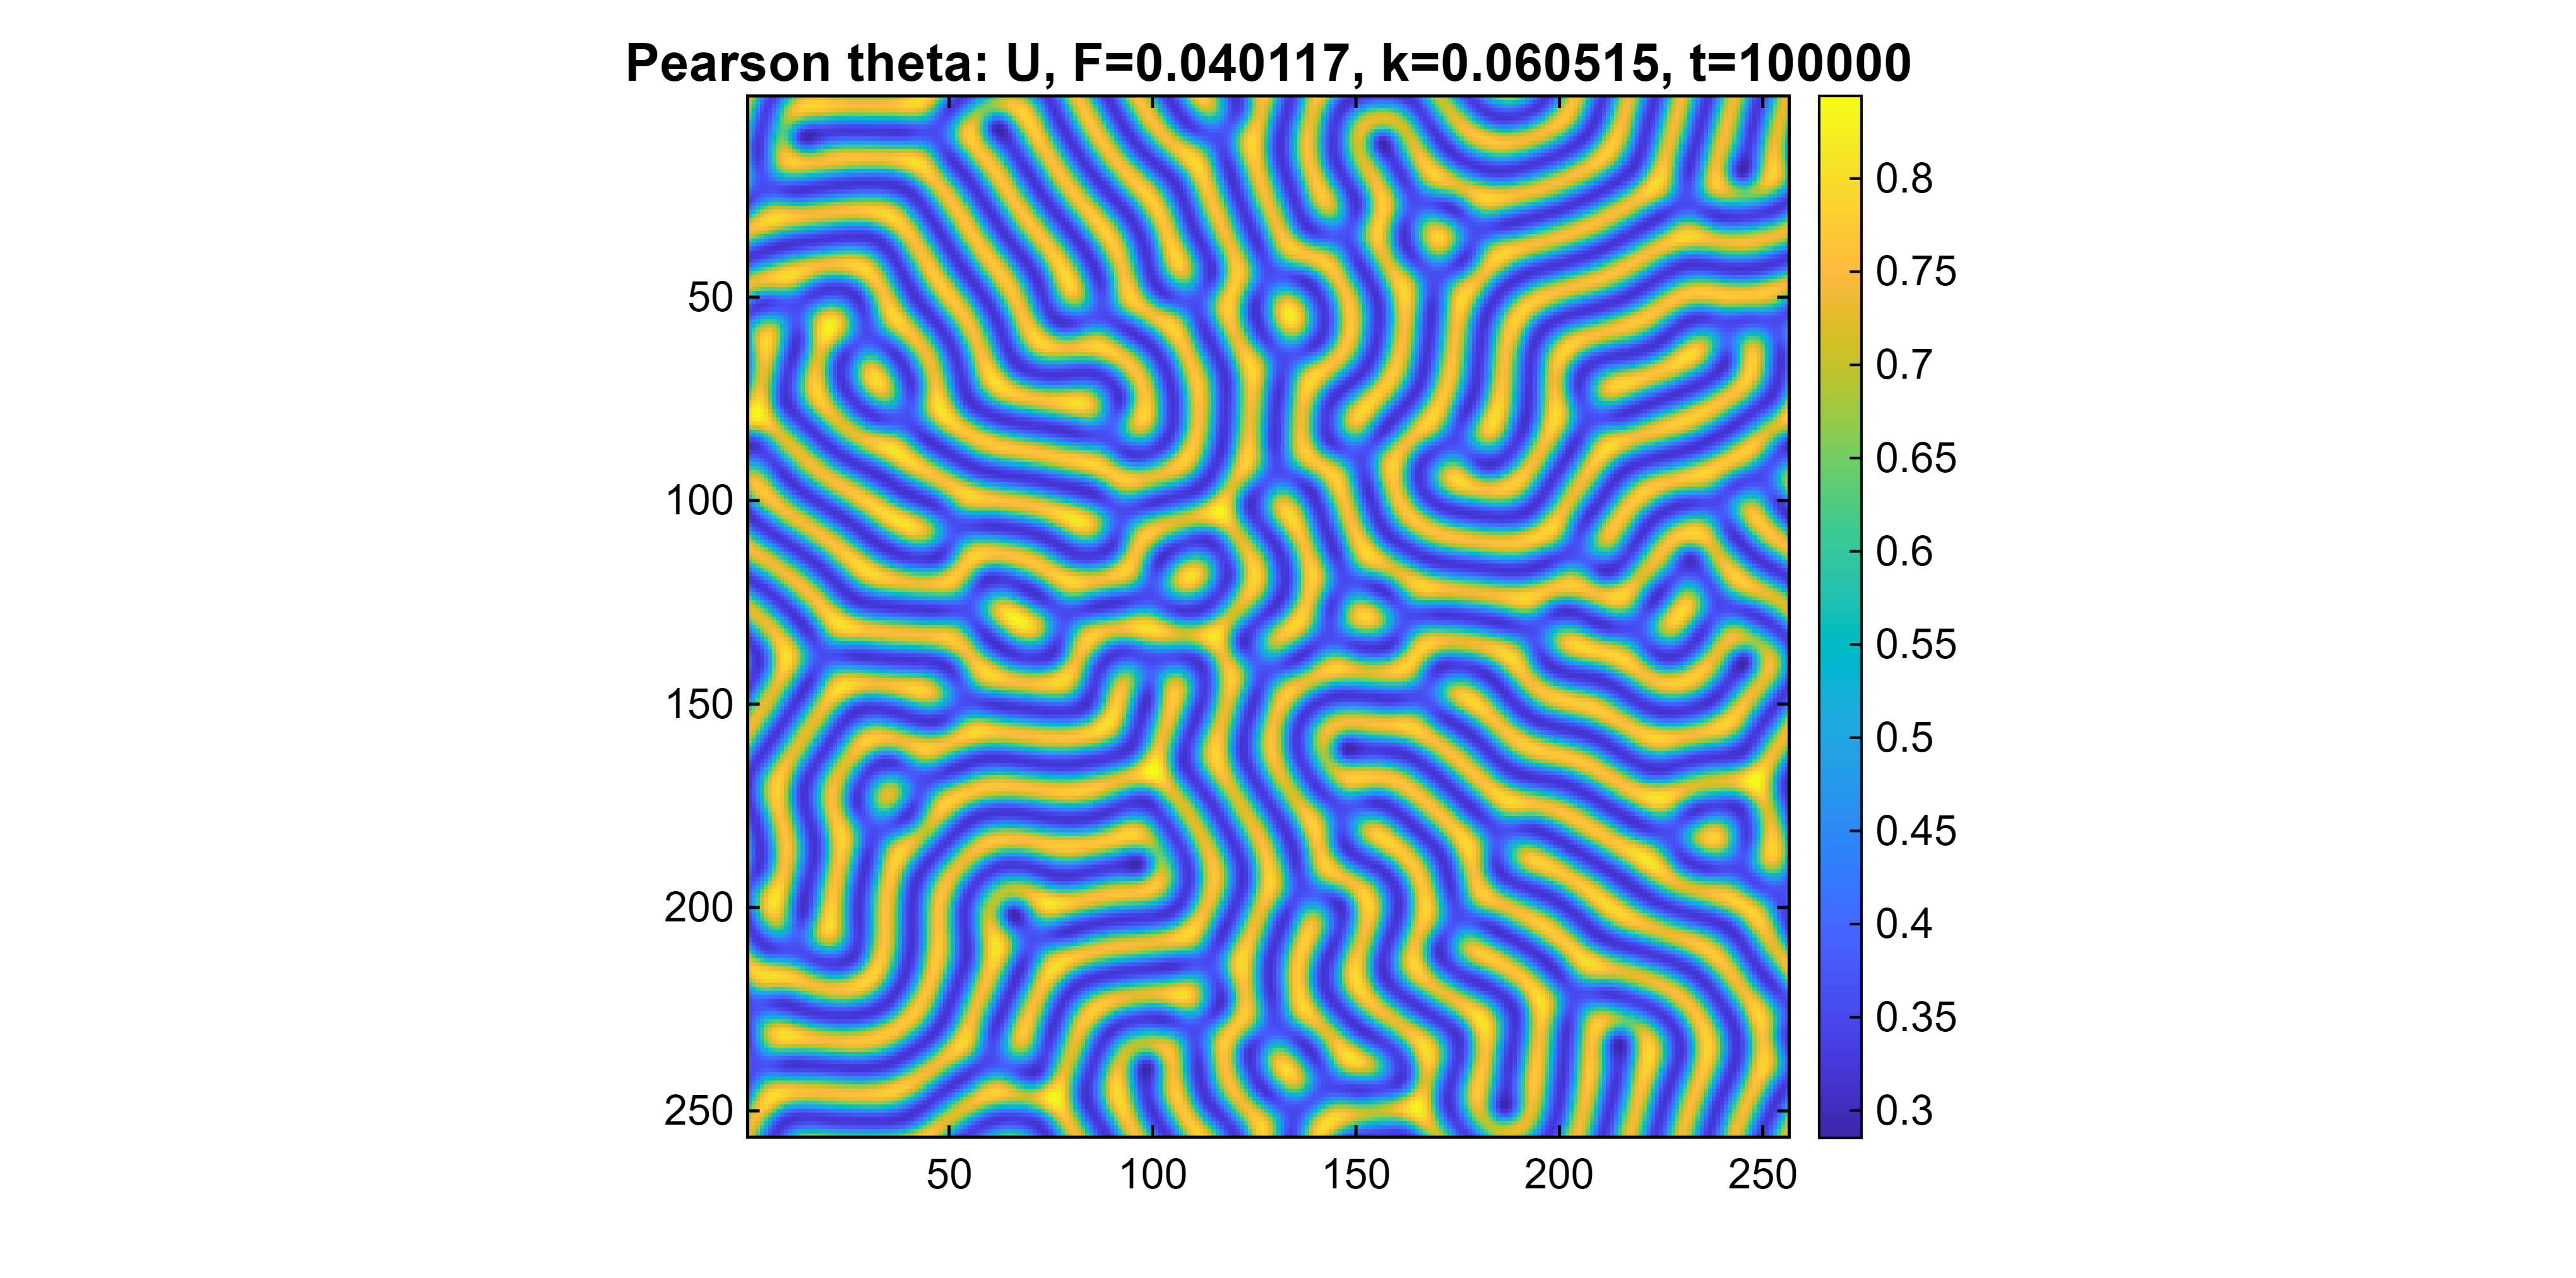
\includegraphics[width=0.95\textwidth]{figures/verification/pattern_sanity/theta_t100000_U.png}
\caption{Pearson \texttt{theta} case: representative \(U\)-field snapshot at \(t=100000\). The pattern is also labyrinth-like, but with a more intricate and locally curved stripe network than in the \texttt{kappa} case.}
\label{fig:pearson_theta_snapshot}
\end{figure}

\section{Verification summary}
\label{sec:verification_summary}

Overall, the verification results show that the implemented Gray--Scott solver behaves consistently with the expected numerical properties of the model and its discretization. The manufactured-solution operator test confirmed second-order spatial accuracy of the discrete Laplacian, while the time-step refinement study confirmed the expected first-order behavior of the explicit Euler method. The boundary-condition tests verified robust enforcement of Dirichlet and Neumann conditions, and the matrix--stencil comparison tests showed that the different diffusion implementations are equivalent both at the operator level and in full end-to-end simulations. In addition, the GUI and non-GUI comparison demonstrated that the graphical interface does not alter the numerical results. The supplementary checks further supported the structural correctness and internal consistency of the implementation. Taken together, these results provide strong verification evidence for the numerical core of the project, while the Pearson-type pattern study offers an additional validation-oriented sanity check at the application level.